%                                                                 aa.dem
% AA vers. 8.2, LaTeX class for Astronomy & Astrophysics
% demonstration file
%                                                       (c) EDP Sciences
%-----------------------------------------------------------------------
%
%\documentclass[referee]{aa} % for a referee version
%\documentclass[onecolumn]{aa} % for a paper on 1 column
%\documentclass[longauth]{aa} % for the long lists of affiliations
%\documentclass[rnote]{aa} % for the research notes
%\documentclass[letter]{aa} % for the letters
%\documentclass[bibyear]{aa} % if the references are not structured
% according to the author-year natbib style


\documentclass{aa}
%LINEBREAKS FOR APPENDIX
\usepackage{array}
%LINEBREAK FOR APPENDIX END
\usepackage{graphicx}
\usepackage{booktabs}
%%%%%%%%%%%%%%%%%%%%%%%%%%%%%%%%%%%%%%%%
\usepackage[varg]{txfonts}
%%%%%%%%%%%%%%%%%%%%%%%%%%%%%%%%%%%%%%%%
\usepackage[draft]{hyperref}
%----bibliograhy stuff----
\usepackage{natbib}
\bibliographystyle{aa}
\bibpunct{(}{)}{;}{a}{}{,}
%%%%%%%%%%%%%%%%%%%%%%%%%%%%%%%%%
%----define citatio aliases ------
\defcitealias{ilin_flares_2019}{PaperI}



% REMOVE AFTER FINISHING DRAFT:

\usepackage{lineno}
\linenumbers

% FINISH REMOVE AFTER FINISHING DRAFT

%---------------------------------
%\usepackage{natbib}
% To add links in your PDF file, use the package "hyperref"
% with options according to your LaTeX or PDFLaTeX drivers.
%
\begin{document}
%LINEBREAKS FOR APPENDIX
\newcolumntype{L}[1]{>{\raggedright\let\newline\\\arraybackslash\hspace{0pt}}m{#1}}
%LINEBREAK FOR APPENDIX END

   \title{Flares in Open Clusters with K2.}

   \subtitle{II. M35, Hyades, and Ruprecht 147}

   \author{Ekaterina Ilin
          \inst{1}, Sarah J. Schmidt\inst{1},
          Katja Poppenhäger\inst{1},
          James R. A. Davenport\inst{2}
          \and
          Klaus G. Strassmeier\inst{1}
          %\fnmsep\thanks{Just to show the usage
          %of the elements in the author field}
          }

   \institute{Leinbiz Institut für Astrophysik Potsdam\\
              \email{eilin@aip.de}
         \and
            University of Washington
             \email{jrad@uw.edu}
             %\thanks{The university of heaven temporarily does not
             %        accept e-mails}
             }

   \date{Received XXX; accepted XXX}

% \abstract{}{}{}{}{}
% 5 {} token are mandatory

  \abstract
  % context heading (optional)
  % {} leave it empty if necessary
   {Flares can help us trace magnetic activity because are bright and high-contrast on low mass stars.}
  % aims heading (mandatory)
   {This study aims to quantify flaring activity on these stars as a function of mass and age.}
  % methods heading (mandatory)
   {We automatically detected flares in K2 time-domain photometry, using the open-source software K2SC to remove instrumental and astrophysical variability from K2 light curves. We used injection and recovery of synthetic flares to assess detection thresholds, time sampling and de-trending effects on the inferred flare energies. With additional data from the full K2 archive we added stars with a larger variety of ages and spectral types to the analysis of the previous study~\citep{ilin_flares_2019}. We compared previous results from the Pleiades and Prasepe to the flare frequency distributions (FFDs) in M35 and the Hyades, respectively. Ruprecht 147 filled in the age gap at 2.5 Gyr between the aforementioned young clusters and the solar age cluster M67.}
  % results heading (mandatory)
   {We find that the flare production mechanism is similar for the entire parameter space, following a power law relation with exponent $\alpha\approx 2$, but the flaring frequencies depend on both mass, and age. We discuss X and Y.}
  % conclusions heading (optional), leave it empty if necessary
   {}

   \keywords{Methods: data analysis, Stars: activity, Stars: flare, Stars: low-mass
               }

   \maketitle

\section{Introduction}
%The impressive morphology of flares has incited our curiosity for decades. Yet the underlying physical processes are still not fully understood on the Sun, and even less so on other stars.
Flares are explosions on stellar surfaces with a complex spatio-temporal and energetic phenomenology. We know that flares are magnetic re-connection events that lead to a change in field line topology and subsequent energy release~\citep{priest_magnetic_2002}. We can observe flares in nearly all electromagnetic bands, from radio %Vilhu et al. 1993, Gudel et al. 1995b,1998, Berger 2002
to X-rays, and on all stars that possess a convection zone, from late F type stars to ultracool dwarfs~\citep{gizis_kepler_2013}. But even with continuous monitoring at high temporal resolution, the random occurrence of solar flares makes them costly observing targets, especially in coordinated multi-band observations. In integrated light, most solar flares have a far too low contrast and intensity to be observable. Stellar flares on cool stars have two advantages in this respect. They are often bright, enhancing stellar flux by up to several orders of magnitude, and they typically exhibit blackbody emission at temperatures significantly higher than their stars' photospheres.
\\
With the evidence that the physical processes that cause flares on the Sun and other stars are the same~\citep{karoff_observational_2016}, solar and stellar flares can inform each other~\citep{shibayama_2013}. Inconsistencies in extrapolations from solar to stellar conditions~\citep{Aarnio2011, aarnio_masslosscme_2012, drake_cmemassloss_2013} provide valuable clues to the differences in magnetic properties between Sun and M dwarfs, too~\citep{alvaradogomez_cme_2018}. Large surveys like Kepler and TESS enable statistical flare studies of stars that were not pre-selected for their activity~\citep{walkowicz_white-light_2011}. Statistical studies of stellar flaring activity can help us understand the underlying physical processes~CITE stellar surface magnetic fields, starspots~\citep{davenport_flaresandspots_2015, howard_evryflare2arxiv_2019}, how flares relate to stellar angular momentum evolution~\citep{mondrik_flarerotation_2019, howard_evryflare2arxiv_2019}, how they affect the atmospheres of exoplanets~\citep{lecavelier_flareescape_2012, loyd_mflaresplanetsfuv_2018, tilley_repeated_flare_2019, howard_evryflare_2019}, and inform galactic archaeology~\citep{howard_evryflare_2019}. %But we also must scrutinize the assumption, and clarify the circumstances under which solar and stellar flares can be related. From G to L
\\
%Flare statistics common sense here ~\citep{lacy_uv_1976}
Basic parameters that affect flaring behaviour on stars are their masses, and ages. Ages can be controlled for in coeval groups of stars, and flaring-age studies in binaries showed consistency in activity for both components in the majority of targets~\citep{lurie_kepler_2015, clarke_flare_2018}. Open clusters present other coeval groups of stars with well-determined ages. \citet{ilin_flares_2019}~(hereafter \citetalias{ilin_flares_2019}) investigated the flaring activity of late-K to mid-M dwarfs in three open clusters (OCs), the Pleiades, Praesepe, and M67, using K2 time domain photometry. They analysed the flare frequency distributions (FFDs), with respect to different masses and cluster ages. For the cluster members, the light curves revealed that their flaring activity declines both with age and mass. The decline is faster for higher mass stars. Recently, \citet{davenport_flaresevolve_2019} put forward an empirical parametrization of this flaring-mass-age relation based on FFDs.
\\
The present study aims to extend the results in \citetalias{ilin_flares_2019} to the age of Ruprecht 147 (2.5 Gyr), and both higher and lower masses than in the previous study. We also test the previous results from the Pleiades on M35, and the results from Praesepe on the Hyades, as both OC pairs have approximately the same ages. Because the Kepler satellite retired in fall 2018, we can now use the complete K2 data set, and supplement all three OCs in~\citetalias{ilin_flares_2019}  with additional light curves. Additionaly, we use high quality K2 light curves available for M67~\citep{nardiello_m67psf_2016} and M35~\citep{soares_furtado_m35_2017}. We discuss our results with respect to potential breaks in the power law distribution at high energies. Finally, we use the results to test the parametrization in~\citet{davenport_flaresevolve_2019}.

 %Guide the reader from a vivid image of a giant flare on a small star to the idea of a flaring clock and OCs as galactic time stamps (blurred by metallicity and other effects).
%How would astronomy benefit from a well-constrained flaring-age-mass relation?
%Detect binary candi
%\textbf{Cool stuff to mention}
%Namekata+2018 found a positive correlation between rotation rate and the speed of starspot emergence and decay, supporting the rotation-flaring relation if flares are produced by starspot dynamics.
%\\

\section{Data}
Our main data are K2 target pixel files that were provided by the Kepler archives hosted at MAST, and light curves derived from them~\citep{aigrain_k2sc_2016, soares_furtado_m35_2017, lightkurve}. To assign $T_\mathrm{eff}$ to the targeted stars we used multiband photometry obtained from Tycho, UCAC4, 2MASS, Pan-STARRS, and Gaia catalogs. To assign ages to the targeted stars,  OC membership information was compiled from the literature. An overview over the cluster sample is presented in Table \ref{data_clusters} and illustrated in Figure \ref{OCs}.

%-------------------------------------------
%--OPEN CLUSTERS DISTANCE AND AGE
%-------------------------------------------
     \begin{figure}
            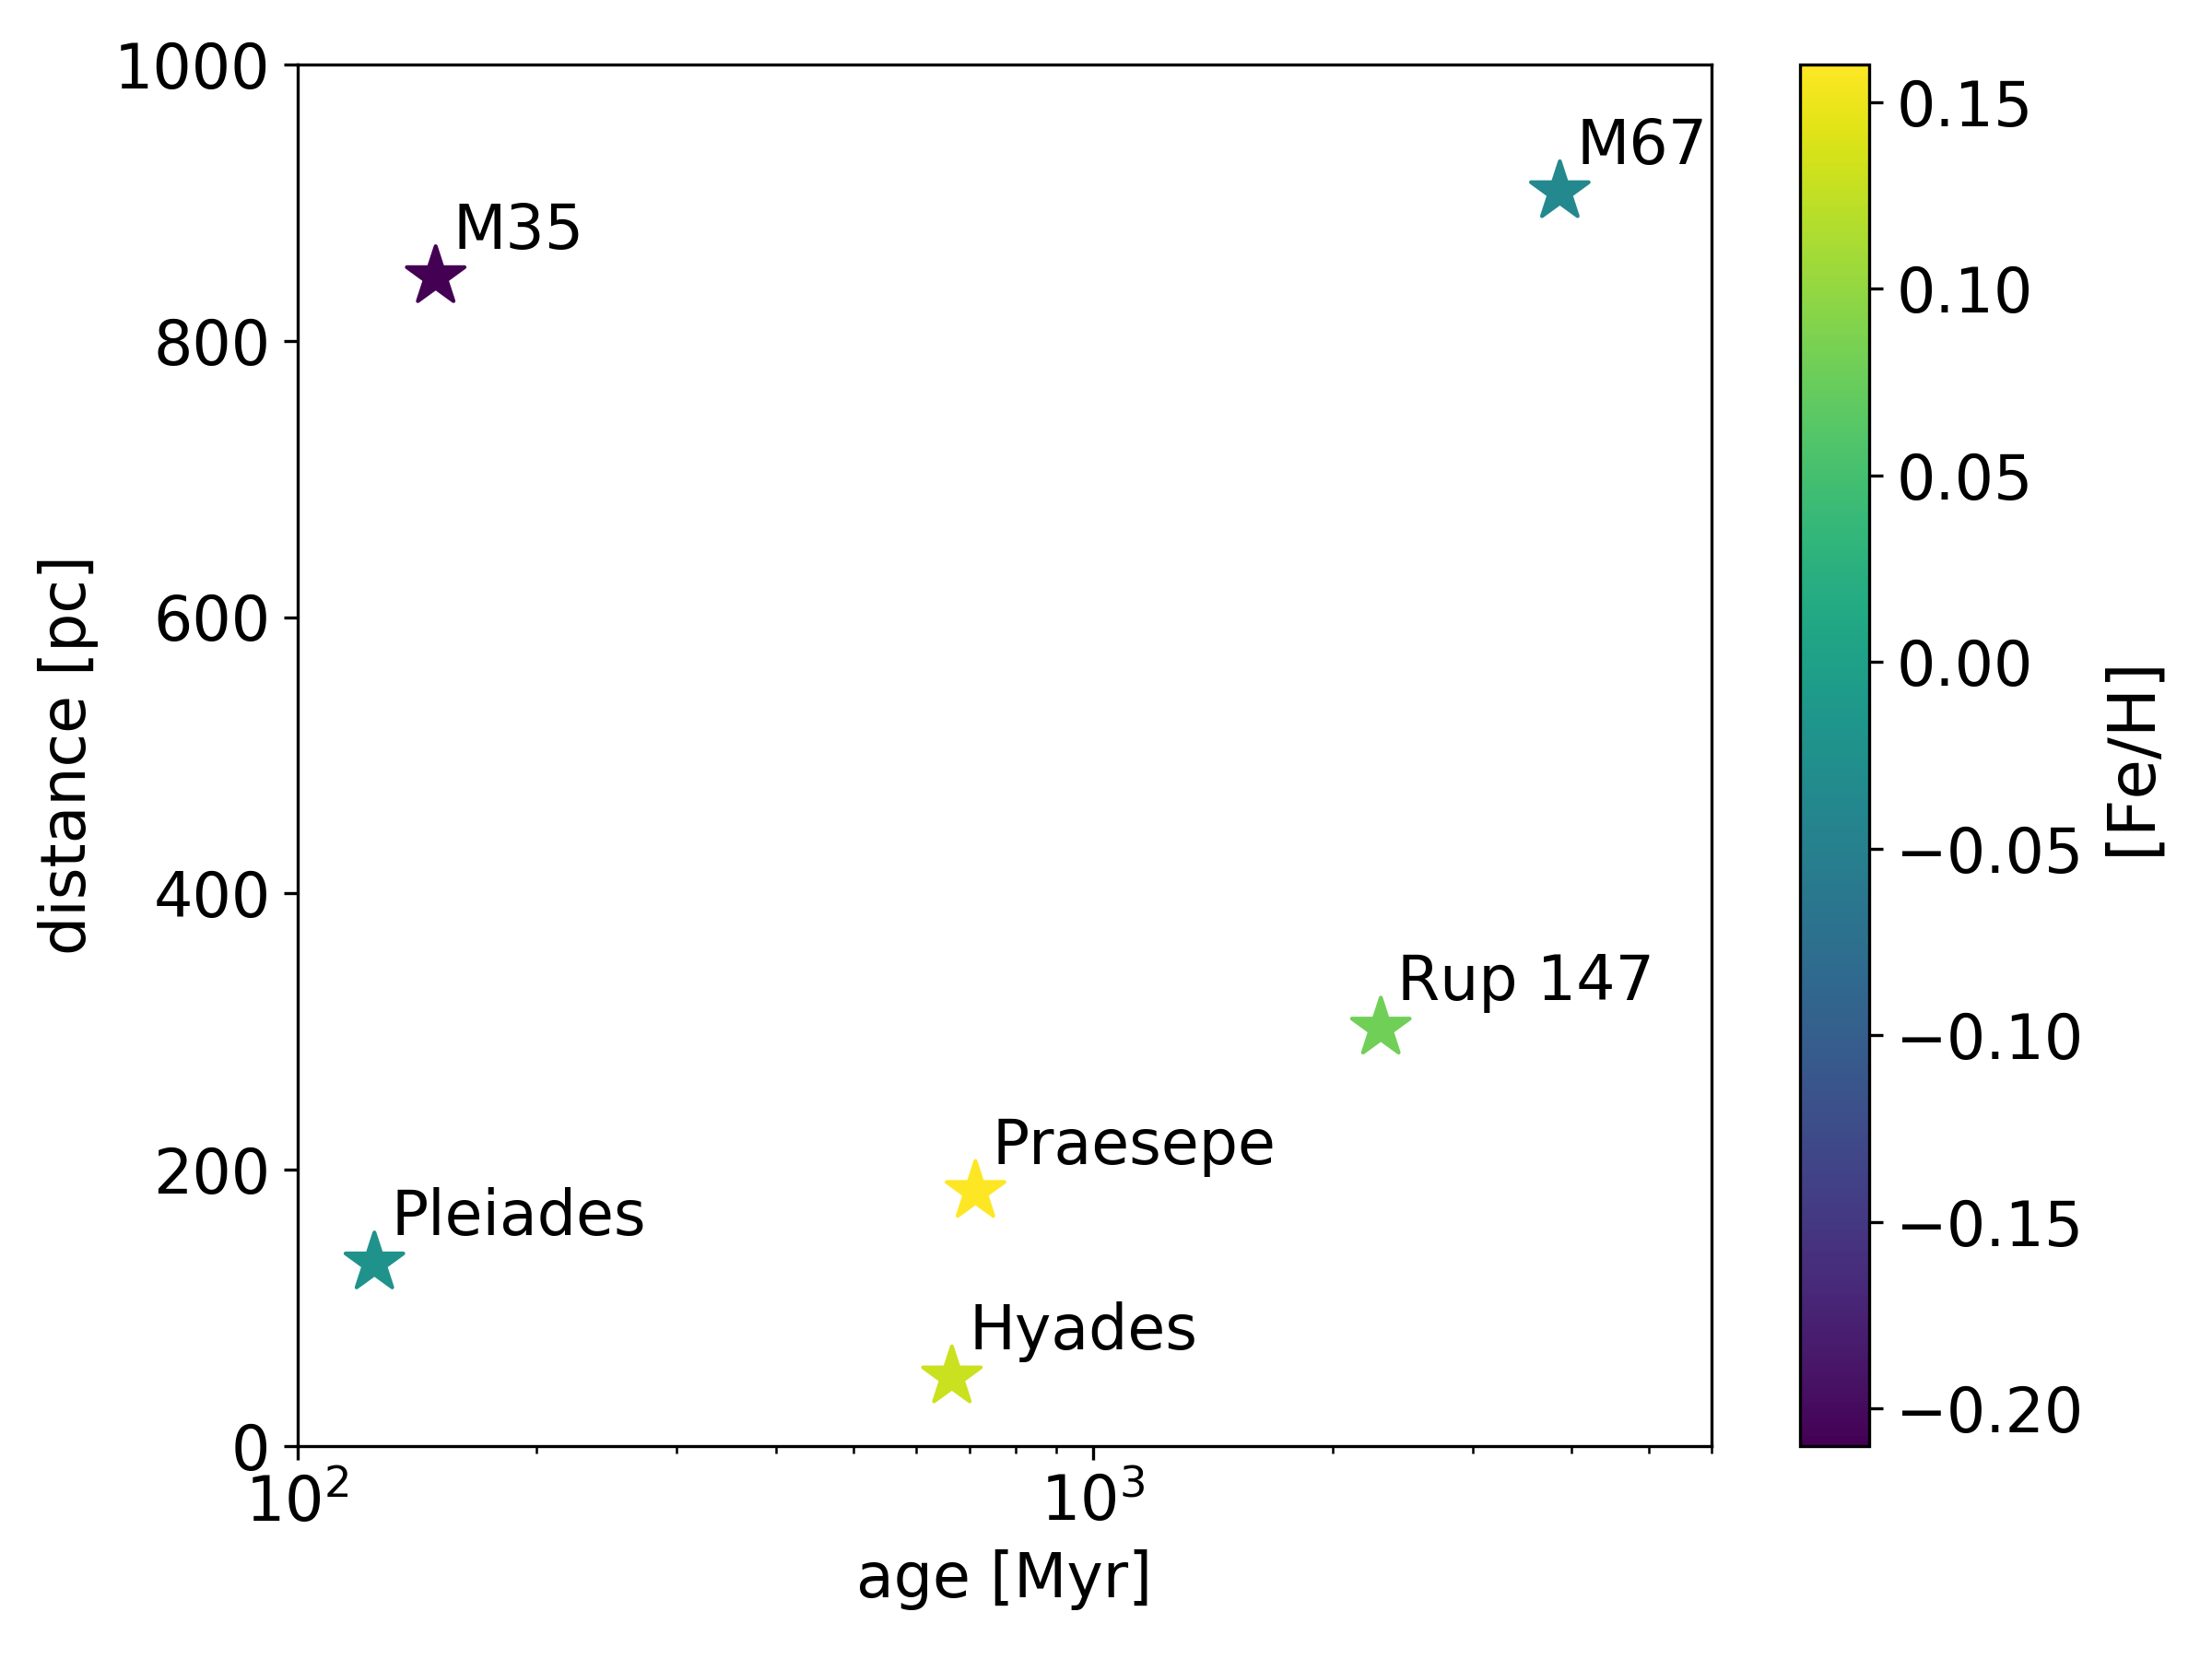
\includegraphics[width=\hsize]{pics/clusters/openclusters_logage_vs_distance.png}
         \caption{The values for age, metallicity, and distance are approximate values from a compilation of existing literature, see Appendix \ref{app_oc_parameters}.}
         \label{OCs}
   \end{figure}

\subsection{K2 light curves}
The Kepler~\citep{koch_kepler_2010} spacecraft finished its follow-up mission K2~\citep{howell_k2_2014} in September 2018, after having completed nearly 20 80-day observing campaigns. Even thought Kepler and K2 data are used in more than 2\,400 publications to date, the public archive can still considered understudied~\citep{barentsen_retirement_opportunities_2018}. In this spirit we took up the analysis of about 4\,000 Kepler target pixel files that each contain up $80$ days of $30$ min cadence observations in white light~($4,200-9,000\,\mathring{A}$). We also used light curves extracted from the K2 C0 super stamp. A super stamp is an aggregated set of typical Kepler postage stamps placed over a densely populated field, that also covered M35~\citep{soares_furtado_m35_2017}.
\\
As K2 was conducted on the two-wheeled Kepler satellite, it was subjected to substantial drift motion (spacecraft roll,~\citealt{van_cleve_thats_2016}) and had an overall reduced pointing accuracy. To mitigate these effects, various solutions were developed~\citep{vanderburg_k2sff_2014, aigrain_k2sc_2016, luger_everest_2016, luger_everst_2018}
\\
%[maybe our own PSF photometry here?]
\subsection{Membership matching}
We obtained membership information from multiple catalogs for each cluster. We cross-matched these catalogs on RA and declination within 3 arcsec. The resulting target lists were used to search the K2 archive, or were matched to the catalogs of extracted light curves from crowded fields in the case of M35~\citep{soares_furtado_m35_2017} and M67~\citep{nardiello_m67psf_2016}.
\\
One part of the membership catalogs provided membership probabilities~\citep{douglas_praesepe_hyades_2014, bouy_messier_2015, cantat_gaudin_2018, olivares_pleiades_2018, reino_hyades_2018, gao_m67mem_2018, olivares_ngc6774_2019}. For the other part no probability was provided~\citep{rebull_rotation_2016, douglas_poking_2017, gaia_dr2_2018_hrd}, or qualitative classifiers were given~\citep{curtis_ruprecht_2013, gonzalez_m67mem_2016,rebull_praesepe_2017}. In the latter cases we assigned approximate probabilities anchored to the set threshold for inclusion into our final sample. Absence in a catalog did not decrease the likelihood of membership, as each catalog shows different selection biases which we did not address in this study. We set the threshold mean membership probability $p$ for a target in our sample to 0.8.
\\
%---------------------------------------------------------------
\subsection{Open Clusters}
%---------------------------------------------------------------
% For the more distant clusters, Ruprecht 147 and M35, we use the mean cluster distance. For the nearby Pleiades, Praesepe, and most importantly the Hyades, we match our targets with Gaia DR2~\citep{gaia_dr2_release_2018} distances, or use mean distances as fallback option. Ages and metallicities are taken from literature, adopting median values when multiple studies were considered, and excluding studies that appear outdated.
We studied flaring activity in the low mass stars in six open clusters spanning from ZAMS to solar age. Table \ref{table_OCs} provides an overview over the final sample. The literature overview of age, distance, and metallicity determinations is given in Table \ref{app0} in the Appendix. Membership probability histograms of the final sample are displayed in Figure \ref{app0_hists}.
\begin{table*}
\caption{Open clusters.}
\label{table_OCs}
\centering
\begin{tabular}{lccccccccr}
\hline\hline
          &  d [pc] &  stars &   LCs &  flares &    campaigns &                        age [Myr] &         [Fe/H] \\
\hline
 Pleiades &   135.6 &    741 &   741 &    1583 &            4 &     $135\left(_{25}^{25}\right)$ &  $-0.04(0.03)$ \\
   Hyades &    46.0 &    170 &   179 &     402 &      , 4, 13 &   $690\left(_{100}^{160}\right)$ &   $0.13(0.02)$ \\
 Praesepe &   185.5 &    913 &  1965 &    1849 &  , 5, 16, 18 &       $750\left(_{7}^{3}\right)$ &   $0.16(0.00)$ \\
  Rup 147 &   305.0 &     53 &    53 &       9 &            7 &  $2650\left(_{380}^{380}\right)$ &   $0.08(0.07)$ \\
      M67 &   908.0 &    234 &   497 &       1 &  , 5, 16, 18 &    $3639\left(_{17}^{17}\right)$ &  $-0.10(0.08)$ \\
\hline

\end{tabular}

\tablefoot{$n$ is the approximate number of members with $p>0.8$. LCs, SLCs, LLCs, and PSF LCs denote the number of available light curves, short cadence light curves, long cadence light curves, and PSF de-detrended light curves, respectively. The values for age, [Fe/H], and distance are approximate values from a comparison of existing literature, detailed in Appendix \ref{app_oc_parameters}.}
\end{table*}
%---------------------------------------------------------------
\subsubsection{Pleiades}
%age distance citation?
The Pleiades, a nearby ZAMS cluster, were observed in Campaign 4, and were treated in \citetalias{ilin_flares_2019}. We include the cluster in this work for completeness and to illustrate improvements to~\citepalias{ilin_flares_2019}. We revisited the memberships from~\citet{rebull_rotation_2016}, which were your in the previous work, and merged them with lists of members determined by~\citet{olivares_pleiades_2018, gaia_dr2_2018_hrd}; and~\citet{cantat_gaudin_2018}.
%---------------------------------------------------------------
\subsubsection{M35}
%age distance citation?
M35 is a ZAMS cluster 900 pc away, observed during Campaign 0 in K2. We merged membership lists from \citet{cantat_gaudin_2018, gaia_dr2_2018_hrd}; and ~\citet{bouy_messier_2015}. There are only five K2 light curves, but we identified multiple additional members with publicly available\footnote{\url{https://k2.hatsurveys.org/archive/}} light curves obtained from \citet{soares_furtado_m35_2017}. They used an image subtraction technique in the campaign's super stamps, a self flat-fielding de-trending inspired by K2SFF~\citep{vanderburg_k2sff_2014}, and a trend-filtering algorithm developed by \citet{kovacs_tfa_algorithm_2005}. We preferred PSF photometry in cases where both aperture K2 and PSF LCs were available. We took the raw extracted PSF light curves and de-trended them using \texttt{K2SC}.
%AMC extracted 1-4 pixel aperture light curves from superstamps in the M35 field, too. We compared the noise levels between the LCs derived from the few-pixel apertures to the PSF case using the median value of a rolling band standard deviation as an estimate.
%---------------------------------------------------------------
\subsubsection{Hyades}
%age distance citation?
The Hyades are a 0.6 Gyr old OC observed during Campaigns 4 and 13 with K2. It is about as old as Praesepe. We merged membership tables obtained from \citet{douglas_praesepe_hyades_2014, reino_hyades_2018}; and \citet{gaia_dr2_2018_hrd}.
%---------------------------------------------------------------
\subsubsection{Praesepe}
%age distance citation?
Praesepe appeared in Campaign 5, and was previously treated in~\citetalias{ilin_flares_2019}. It was then observed again during Campaign 13. We revisited the memberships obtained by \citet{douglas_praesepe_hyades_2014}, and matched them to the members identified in \citet{douglas_poking_2017, rebull_praesepe_2017,cantat_gaudin_2018}; and ~\citet{gaia_dr2_2018_hrd}.
%---------------------------------------------------------------
\subsubsection{Ruprecht 147}
%age distance citation?
Ruprecht 147 is a 2.5 Gyr old OC observed during Campaign 7 with K2. We used the mean membership probabilities obtained from a number of studies~\citep{curtis_ruprecht_2013, cantat_gaudin_2018, olivares_ngc6774_2019} combined with the members found by~\citet{gaia_dr2_2018_hrd} to identify the most likely members.
%---------------------------------------------------------------
\subsubsection{M67}
%age distance citation?
% how were the Nardiello LCs treated?
M67 is a solar-age, solar metallicity OC about 900 pc away. Multiple members were observed during Campaign 5, and revisited in Campaigns 16 and 18. We did not find any flares in M67 in Campaign 5~\citepalias{ilin_flares_2019} observing the members identified by \citet{gonzalez_m67mem_2016}. The recent campaigns brought both additional observations, and entirely new targets to the sample. We merged the members from \citet{gonzalez_m67mem_2016} with a recent study based of Gaia DR2 data~\citep{gao_m67mem_2018}. Additionally, we obtained PSF-detrended light curves for Campaign 5 from~\citet{nardiello_m67psf_2016}.
%---------------------------------------------------------------
\subsection{Effective temperatures, stellar radii, and luminosities}
\label{TeffRL}
%---------------------------------------------------------------

%---------------------------------------------------------------
% CTRs
%---------------------------------------------------------------

   \begin{figure*}
		\centering
           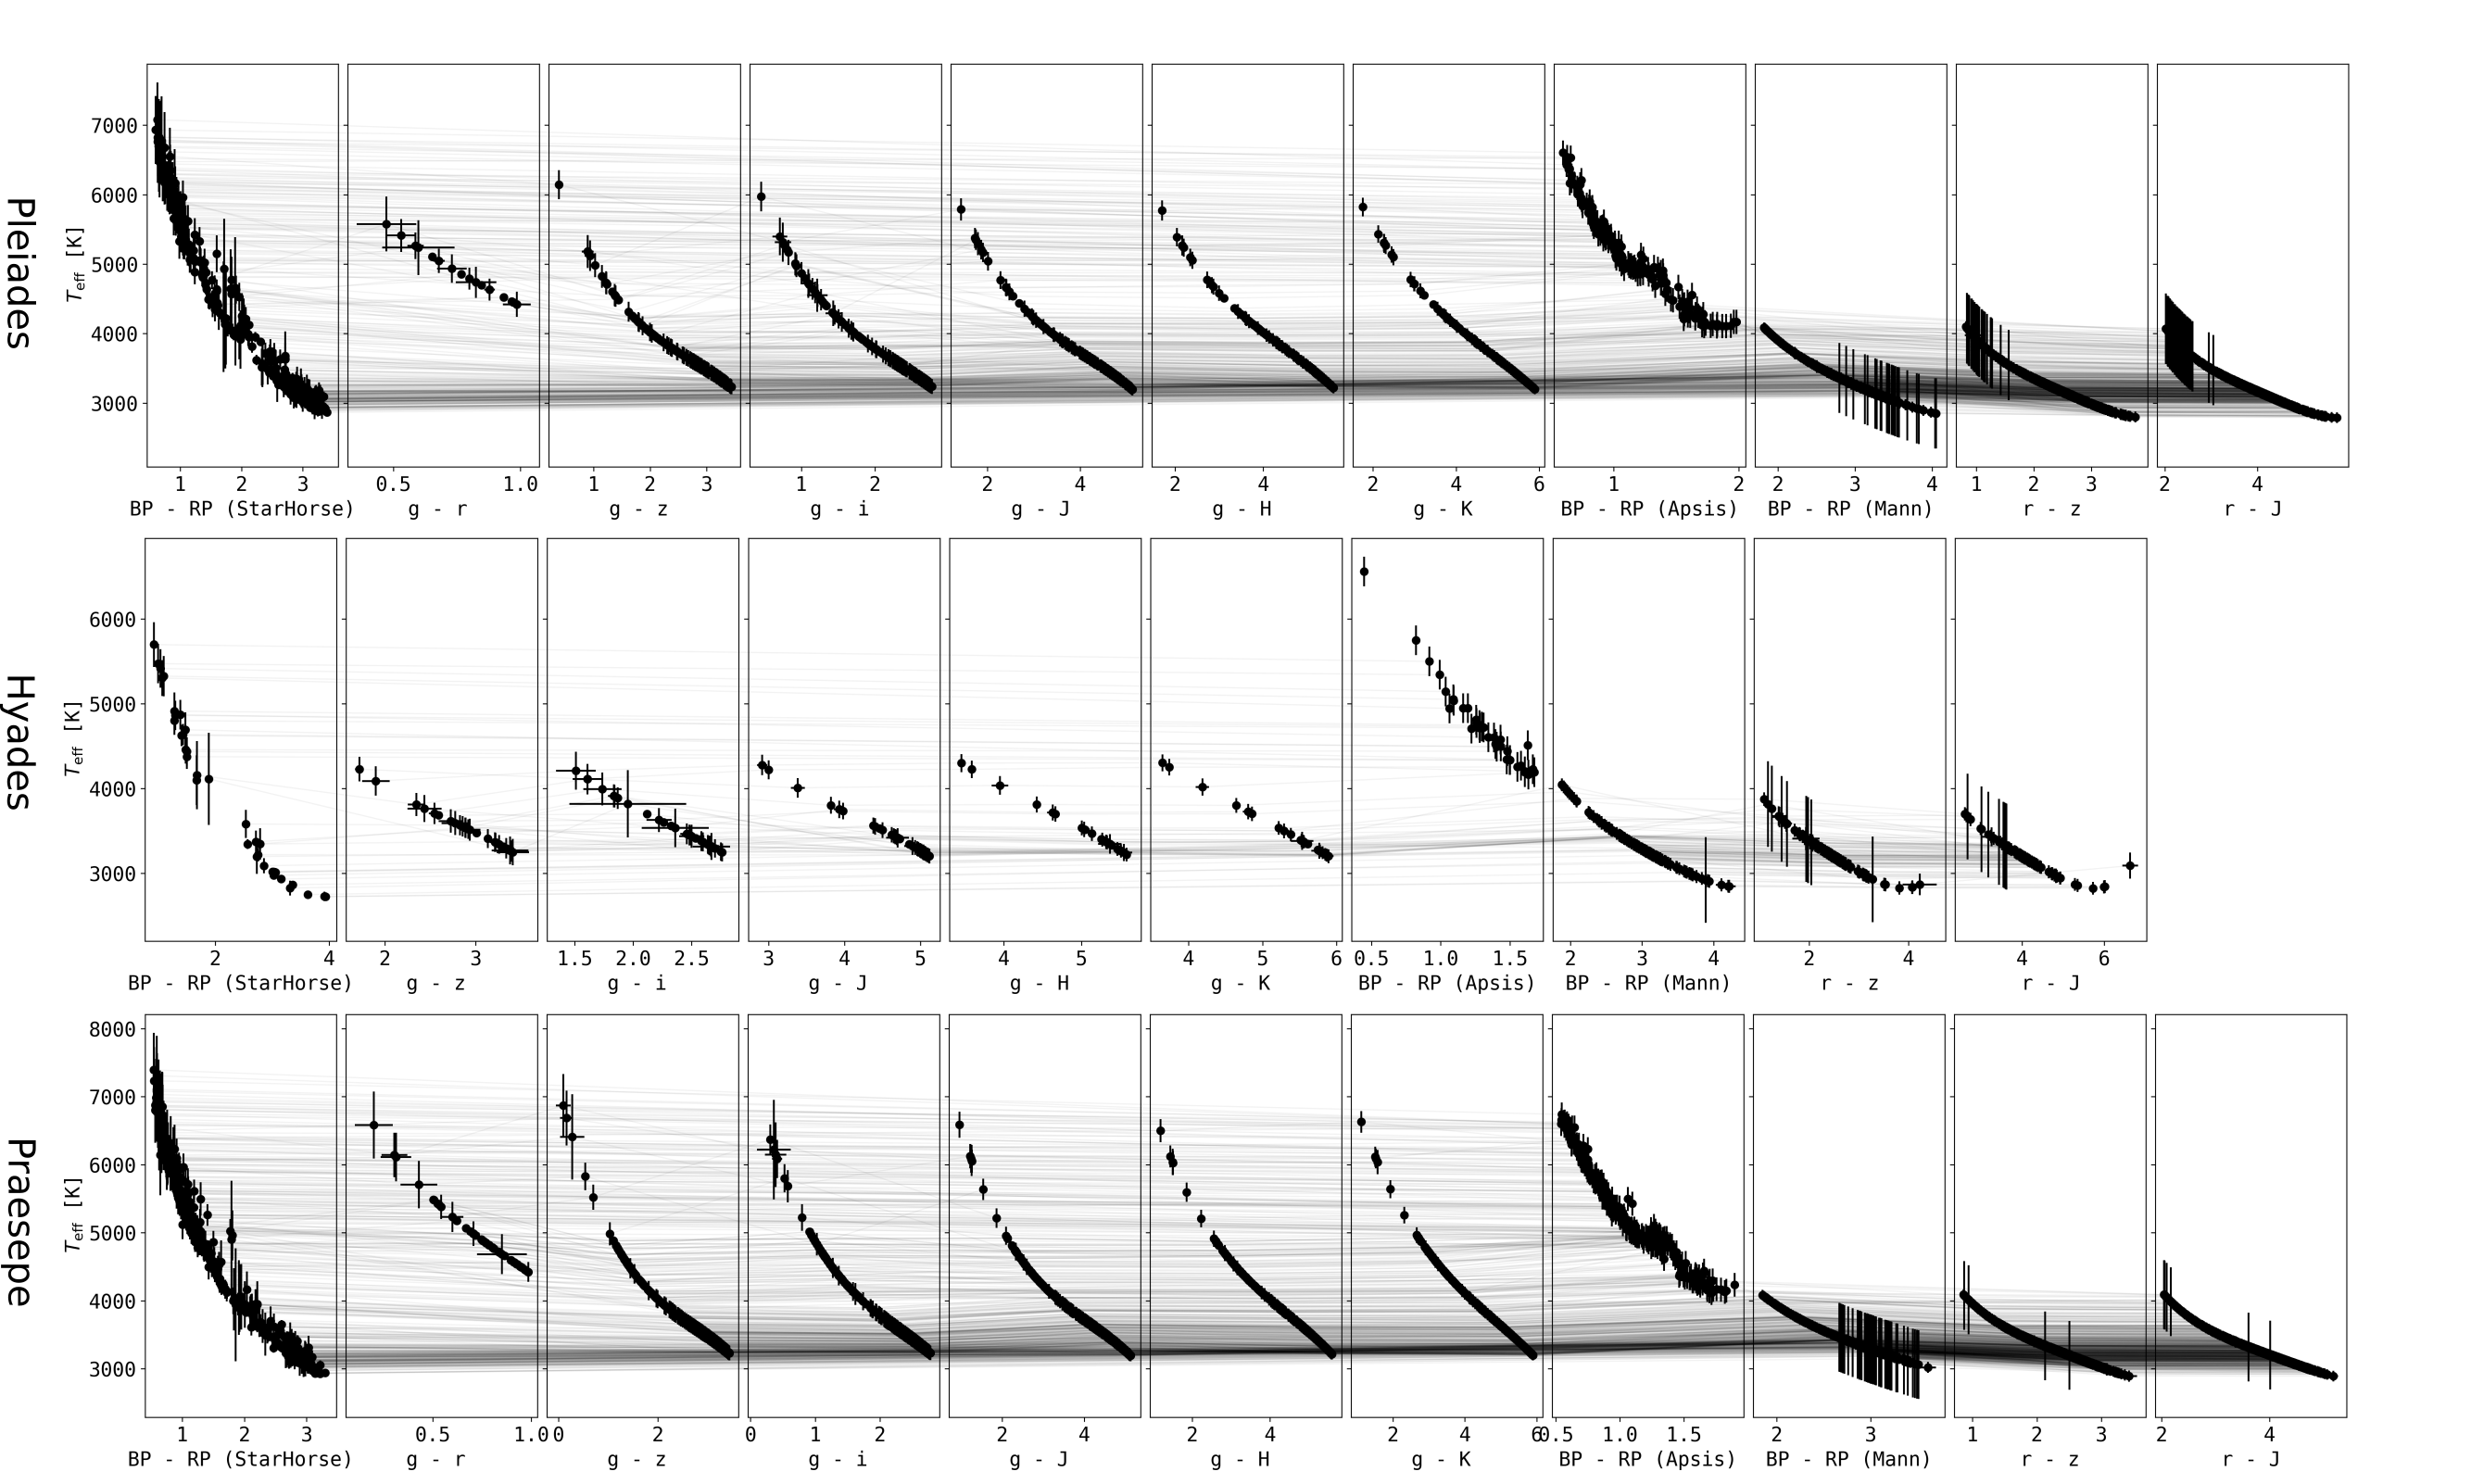
\includegraphics[angle=90, width=0.8\hsize]{pics/clusters/Teff_spread_young.png}

      \caption{Color-temperature relations for Pleiades, M35, and Hyades.  }
         \label{pleiades_m35_hyades}
   \end{figure*}
   

   \begin{figure*}
		\centering
           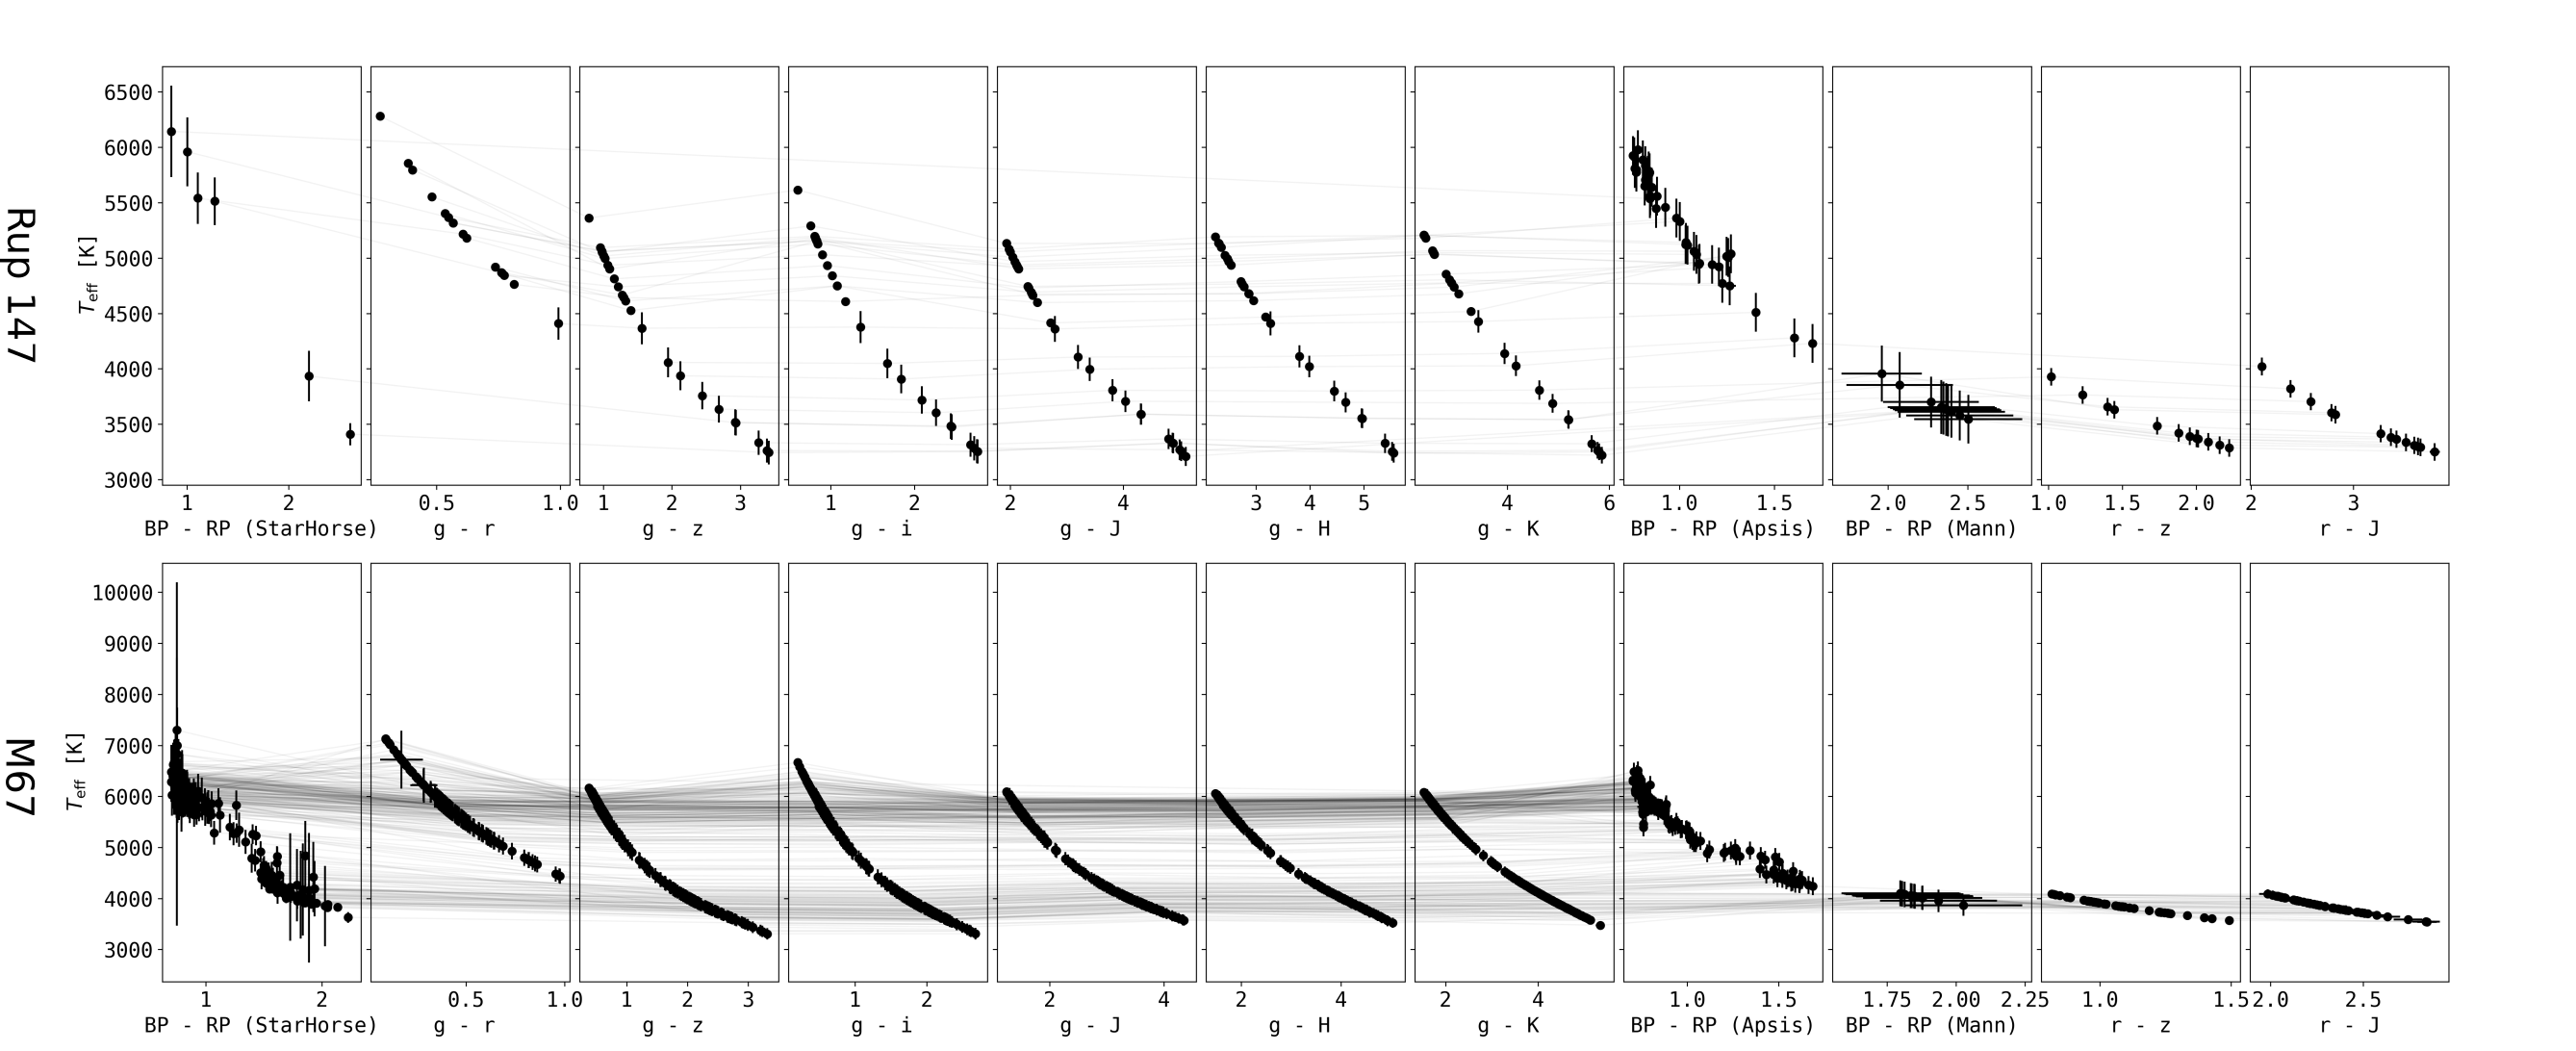
\includegraphics[angle=90, width=0.56\hsize]{pics/clusters/Teff_spread_old.png}

      \caption{Color-temperature relations for Praesepe, Ruprecht 147, and M67. Description as in Fig. \ref{pleiades_m35_hyades}.}
         \label{praesepe_ngc6774_ngc2682}
   \end{figure*}   
%---------------------------------------------------------------
%---------------------------------------------------------------

%---------------------------------------------------------------
% Teff - R
%---------------------------------------------------------------


   \begin{figure*}
		\centering
           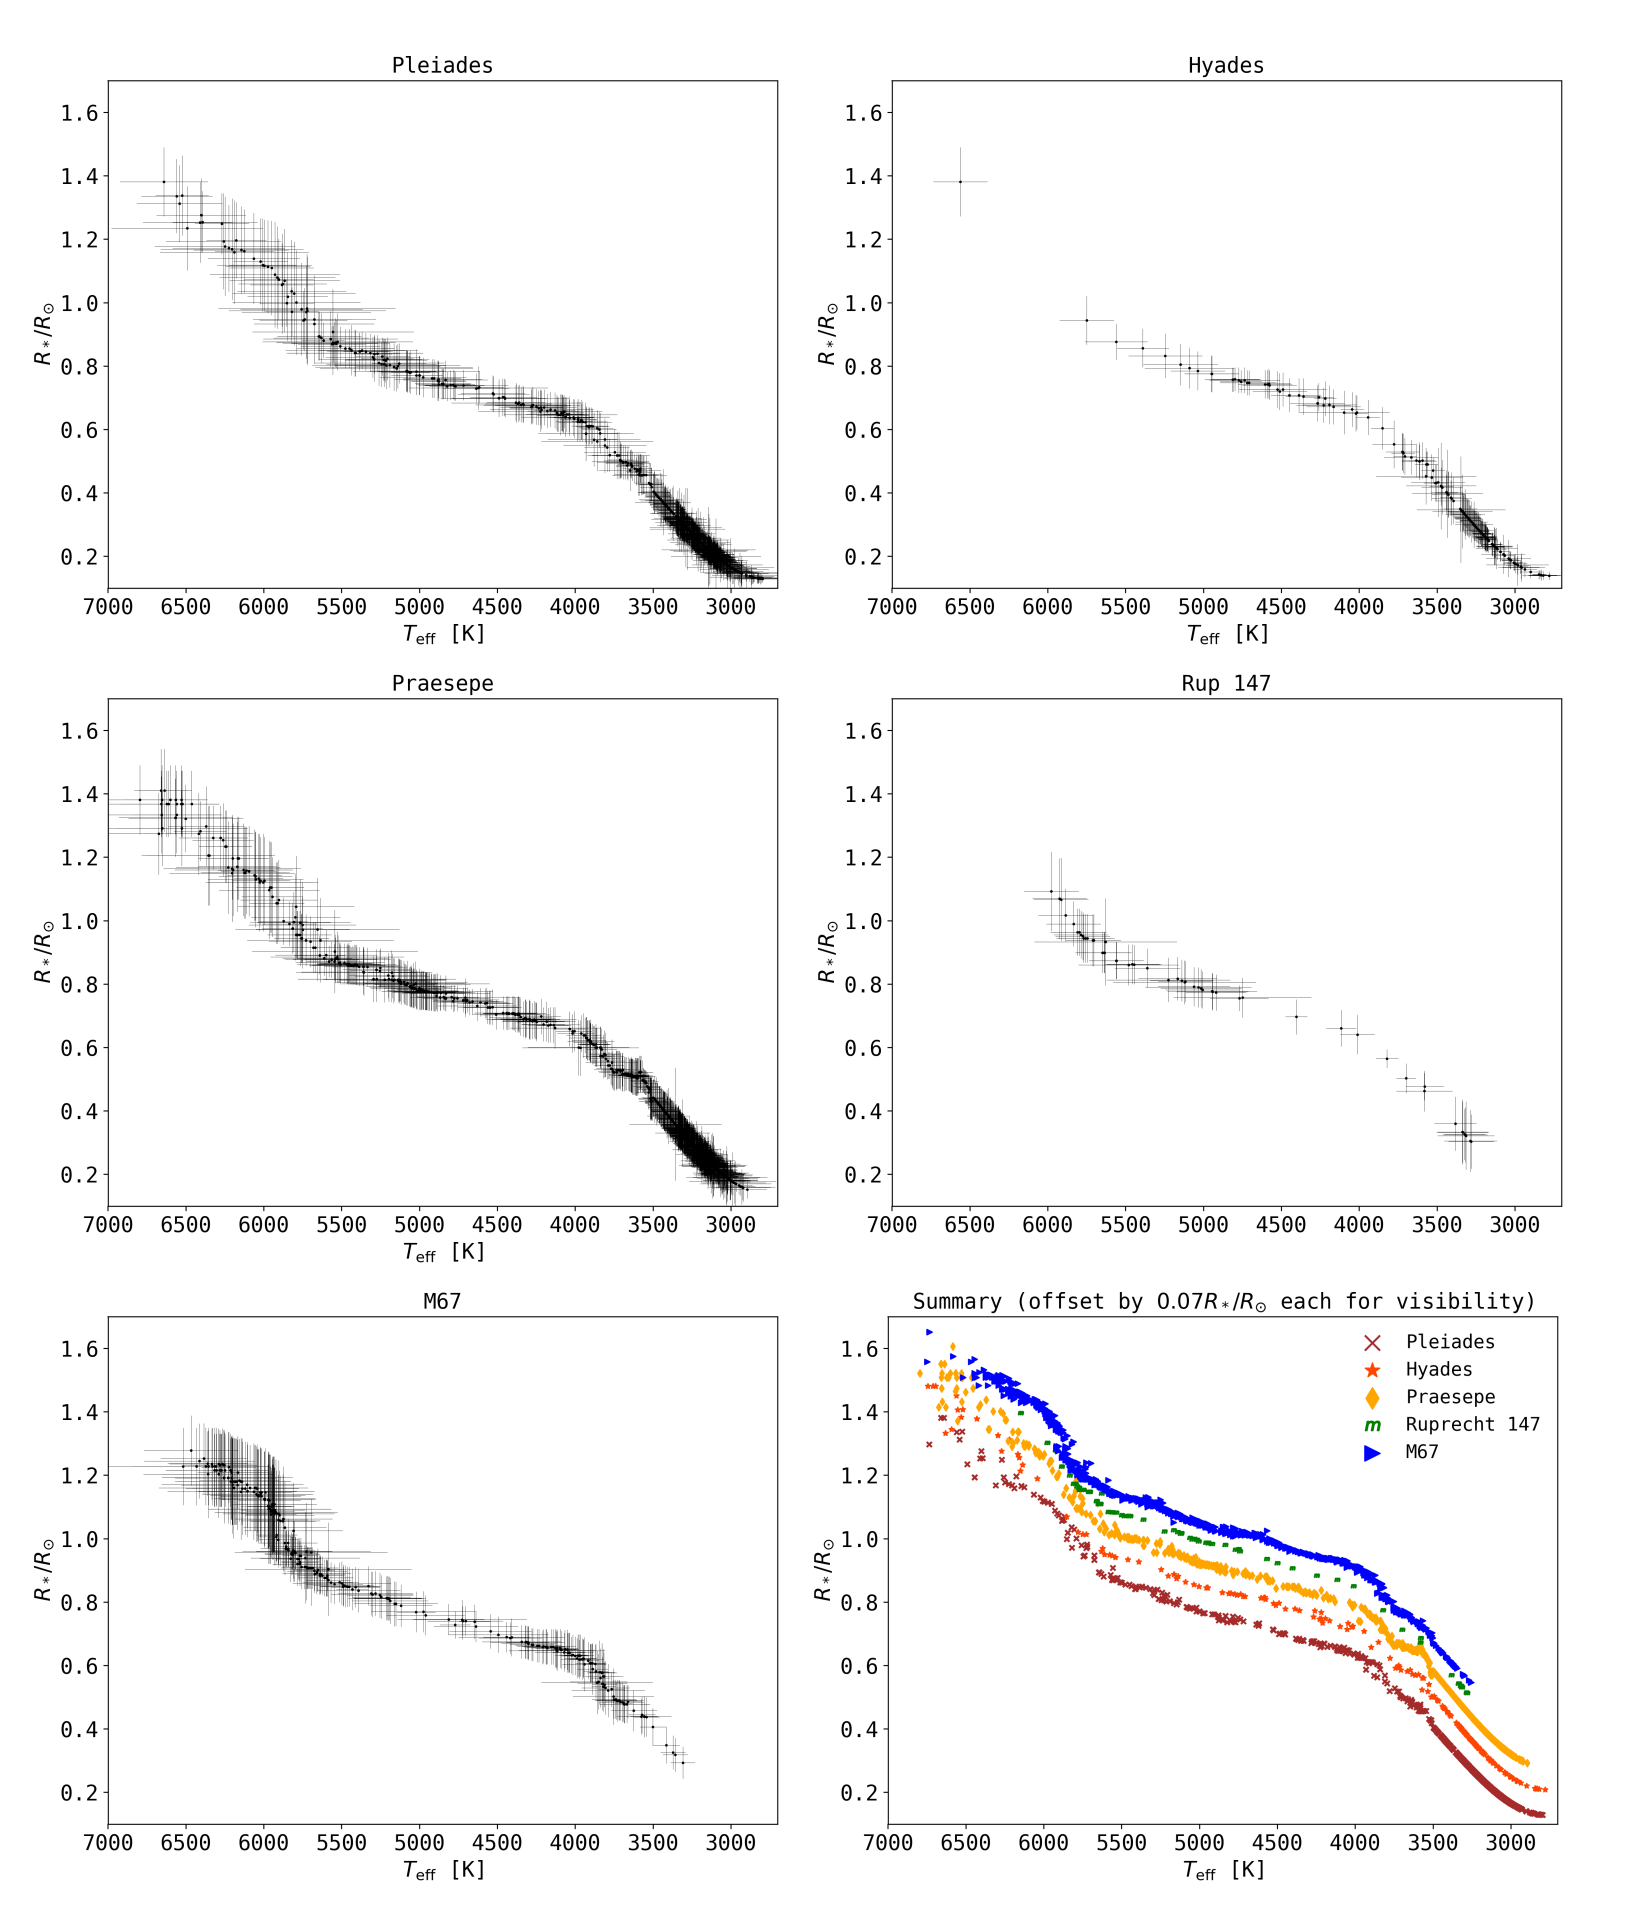
\includegraphics[width=\hsize]{pics/clusters/teff_R.png}

      \caption{$T_\mathrm{eff}-R_*$ relation for all clusters in this study.}
         \label{teff_R}
   \end{figure*}   

%---------------------------------------------------------------
%---------------------------------------------------------------

\subsubsection{Photometry and extinction correction}
We determined effective temperatures $T_\mathrm{eff}$ using broadband photometry the Two Micron All Sky Survey~(2MASS; \citealt{skrutskie_two_2006}), the Panoramic Survey Telescope and Rapid Response System \mbox{(Pan-STARRS)} Data Release 1~\citep{2016arXiv161205560C}, and Gaia DR2~\citep{gaia_dr2_release_2018}. We applied quality cuts to 2MASS, Pan-STARRS DR1, and GaiaDR2 data, as described in Appendix \ref{appendix_photometry}, and removed foreground stars using Gaia DR2 parallaxes. We corrected the 2MASS and PanSTARRS photometry in M35, M67, and Ruprecht 147 for extinction using the most recent version~\citep{green_bayestar_2019} of the \texttt{dustmaps} package that provides 3D dust maps derived from 2MASS and PanSTARRS photometry together with Gaia distances~\citep{green_dustmaps_2018}. If there was no Gaia parallax available we used the cluster median distance instead. If an extinction value was not available for a given star we used the average extinction value of the respective cluster. We accounted for extinction in Gaia BP and RP using the reddening $E(B_P-R_P)$ derived from Gaia photometry and parallax from Gaia DR2~\citep{andrae_gaiaapsis_2018}. We dropped targets that were too bright (Kepler magnitude $K_\mathrm{p} \leq 9$).
%The latter were obtained using TOPCAT~\citep{Taylor_TOPCAT_2005}\footnote{\url{http://www.star.bristol.ac.uk/~mbt/topcat/}}.
\\

\subsubsection{Effective temperatures}
We applied several methods and color-temperature relations (CTRs) to determine robust $T_\mathrm{eff}$. We used CTRs from \citet{boyajian_stellar_2013} and \citet{mann_erratum_2016} (erratum to \citealt{mann_how_2015}), and $T_\mathrm{eff}$ derived from Gaia DR2 using the StarHorse algorithm~\citep{queiroz_starhorse_2018} and inferred from Gaia DR2 using the Apsis pipeline~\citep{bailerjones_apsis_2013, andrae_gaiaapsis_2018}.
\\
\citet{boyajian_stellar_2013} determined CTRs from a range of interferometrically characterized stars using $g-z$, $g-i$, $g-r$, $g-J$, $g-H$, and $g-K$ colors from SDSS and Johnson magnitudes for A to K stars. Their sample is centered on solar metallicity, so we constained the use of these CTRs to stars with $-0.25<$\,[Fe/H]$\,<0.25$. We transformed 2MASS JHK to $J-H$, $H-K$, and $J-K$ in the Johnson system  as the authors from 2MASS to the Bessell-Brett sytem~\citep{carpenter_color_2001}, and from Bessell-Brett to Johnson using the relations in~\citet{bessell_brett_1988}. 
\\
\citet{mann_how_2015} provide CTRs from absolutely calibrated spectra to which they fitted atmospheric models to obtain $T_\mathrm{eff}$. Alternatively, they determined $T_\mathrm{eff}$ from long-baseline optical interferometry measurements using the bolometric flux. Among others, they note transformations for SDSS/2MASS $r-z$ and $r-J$, or Gaia $BP-RP$ where extra information can be added from metallicity or 2MASS $J-H$. The relations in \citet{mann_how_2015} are only valid if metallicity is sufficiently close to solar, which is satisfied for all clusters in this paper~(see Table \ref{data_clusters}). M35 may be an exception to this rule.
\\
We supplemented our estimates with $T_\mathrm{eff}$ estimates from \citet{anders_starhorse_2019} who used the StarHorse pipeline~\citep{queiroz_starhorse_2018} on Gaia DR2.
\\
Gaia DR2 published effective temperatures for over 160 million sources~\citep{gaia_dr2_release_2018}. The typical uncertainty is quoted at 324 K, but it is lower for stars above $\sim$4100 K and below $\sim$6700K, so that we adopt 175 K which is above the quoted root-median-squared error in this $T_\mathrm{eff}$ range~\citep{andrae_gaiaapsis_2018}, and use provided values only in this range.
\\
Empirical CTRs suffer from systematic errors that stem both from the different methods applied, and from sample selection biases. We used as many empirical relations as possible in their appropriate ranges to obtain multiple $T_\mathrm{eff}$ estimates from which we then drew a more reliable median value. Targets that were lacking sufficient photometric data to derive $T_\mathrm{eff}$, or were too hot to be expected to have a convective envelope ($T_\mathrm{eff} \geq 7000$;K), were flagged accordingly, and removed from the sample. We dropped all targets where the uncertainty on the weighted mean $T_\mathrm{eff}$ was greater than 10\%. Only targets that were assigned a $T_\mathrm{eff}$ were searched for flares. 
%what are the distributions of uncertainties on Teff
\subsubsection{Stellar radii}
We used a catalog of empirically characterised stars~\citep{yee_specmatch_2017} to derive $R_*$ from $T_\mathrm{eff}$ (Fig.~\ref{teff_R}). \citet{yee_specmatch_2017} collected 404 stars with high-resolution spectra from the literature, and own observations of mid to late K-dwarfs, spanning low mass stars from 7000\;K down to 3000\;K. For these stars, the resulting catalog is accurate to 100\;K in
$T_\mathrm{eff}$, 15\;\% in $R_*$, and 0.09\;dex in [Fe/H]. We interpolated between stars from the catalog to our derived $T_\mathrm{eff}$,  and propagated the resulting scatter to the uncertainty in $R_*$ if $T_\mathrm{eff}>3500$ K. For stars with $T_\mathrm{eff}< 3500$ K we used $T_\mathrm{eff}-R_*$ relations derived by~\citep{mann_how_2015,mann_erratum_2016}.
\subsubsection{Spectra}
We assigned spectra to our targets from the SpecMatchEmp~\citet{yee_specmatch_2017} and the FlareSpecPhot libraries~\citep{Schmidt2014b,Kirkpatrick2010, Burgasser2007,Burgasser2008,Burgasser2010, Burgasser2004,Cruz2004, Burgasser2006, Rayner2009, Doi2010, Filippazzo2015, Cruz2003, West2011, Bochanski2010,  Bochanski2007, Schmidt2010, Schmidt2015, Schmidt2014a, mann_how_2015}. When a specturm was available for the derived spectral type in FlareSpecPhot, we preferred it over SpecMatchEmp, which was the case for all stars cooler than M0, where we mapped spectral type to effective temperature as appears in~\citet{pecaut_intrinsic_2013}. We then combined stellar radii $R_*$, $T_\mathrm{eff}$, and spectra to projected bolometric luminosities $L_{\mathrm{bol,*}}$, and projected luminosities in the Kepler band $L_{\mathrm{Kp,*}}$~\citep{shibayama_superflares_2013,ilin_flares_2019}. Uncertainties on $L_{\mathrm{Kp,*}}$ ranged from 9\;\% to 52\;\% with a median value of 17\;\%.
%uncertainties on derived luminosities
%\citet{rabus_discontinuity_2019} found a discontinuity in the Teff-R relation to occur around 0.23 $M_{\odot}$, and a corresponding bimodal distribution of stellar radii from $T_\mathrm{eff}$ between 3200 and 3340 K. Estimates of bolometric luminosity based on $R$ derived from $T_\mathrm{eff}$, even using empirical relations, can then be off by factors of 2 to 6. While estimates of $M_*$ can help lift this degeneracy they are not provided independently in our sample. We would then have to acknowledge the increased uncertainty in the luminosities for the stars that fall in this regime. However, the observed transition is consistent with very low mass stellar models, where it is not a break but a smooth transition in the Teff-R relation caused by the non-linear increase in the core electron degeneracy parameters with decreasing stellar mass~\citep{cassisi_nodiscontinuity_2019}. %can we account for it
\section{Methods}
We detected flare candidates automatically, and validated them by eye. We attempted to assign recovery probabilities and corrected for sampling effects using injection/recovery tests but the procedure was not scalable due to computational costs. We performed injection recovery on a handful of example light curves to see that de-trending and intrinsic light curve properties smear out the $ED$ recovery with varying distributions that add an uncertainty of about 30\%. Most of the candidates are expected to have a complex shape that deviates from the classical flare template. The validation yielded an estimate on the uncertainty on the flare energy released in the Kepler band. The frequency distributions of these flare energies are believed to follow a power law that spans multiple orders of magnitude. We adopted this model, and used two different Maximum Likelihood estimators to obtain the power law exponents. We tested the best fit parameters with the Kolmogorov-Smirnov test, and probed possible truncation of the power law relation with an exceedance test.
\subsection{Flare finding}
We used the open source software \texttt{AltaiPony}\footnote{\url{https://github.com/ekaterinailin/AltaiPony}} to automatically detect and characterize flares in our sample. The code base relies on \texttt{K2SC}\footnote{\url{https://github.com/OxES/k2sc}}~\citep{aigrain_k2sc_2016} to remove instrumental and astrophysical variablity from K2 light curves. We did not use the pre-detrended light curves available on MAST, but used \texttt{K2SC} to derive our own, because we clipped outliers at $3\sigma$ iteratively, as compared to the original work, where outliers were clipped at $5\sigma$~\citep{aigrain_k2sc_2016}.
\\
After de-trending, the flare finder algorithm looked for continuous observing periods, defined as being longer than 10 data points at a minimum cadence of 2\;h. All further routines were run on these observing periods. The finder iteratively clipped excursions from the median value at $3\sigma$ rolling window noise above median plus uncertainty given from \texttt{K2SC} de-trending. After each iteration, outliers were cut down to the current median value. Either after convergence, or 50 iterations, the resulting median value was adopted. With this median as quiescent flux, flare candidates were identified with the same procedure as during the median value calculation, but now we additionally required at least three consecutive data points to fullfil the $\sigma$-criterion. Flare candidates were merged into single candidate events if they were no more than three data points apart. For each of these candidates occurrence time, amplitude and equivalent duration ($ED$) was returned.
\\
The Kepler flare sample has shown to be difficult to treat in a fully automated way. Without manual vetting, the event samples remain significantly contaminated~\citep{yang_keplerflares_2019}. 
\\
$ED$ is the area between the LC and the quiescent flux, that is, the integrated flare flux divided by the median quiescent flux $F_0$ of the star, integrated over the flare duration~\citep{hunt-walker_most_2012}:
\begin{equation}
\label{05_ED}
ED=\displaystyle \int \mathrm dt\, \frac{F_{flare}(t)}{F_0}.
\end{equation}
$ED$ is a quantity independent of calibration and distance that is suited to compare flaring activity on stars where these properties are uncertain. It describes the time during which a star releases as much energy as the flare itself. This time can be shorter or longer than the actual flare duration. 
\\
The uncertainty in $ED$ depends on the light curve noise properties, time sampling, and other intrinsic characteristics. Moreover, K2SC de-trending and the flare finding procedure introduce additional uncertainty that dominates the photometric noise. Carrying out injection and recovery that takes into account the effect of GP regression that underlies K2SC. We only performed injection-recovery on a small number of light curves with flares to estimate the .  
%\subsection{Recovery probability and $ED$ correction}
%\label{recprob_edcor}
%To further validate the flare events, every candidates was re-injected to its light curve of origin several times with varying amplitude and duration using a classical flare template~\citep{davenport_kepler_2014}. This returned a recovery probability of similar flare morphologies on a given light curve. We accepted a candidate if the recovery probability was above 80\;\%. From the difference between injected and recovered values we calculated individual correction factors for all candidates that typically increased the $ED$ because the 30\;min time sampling systematically underestimates the $ED$~\citep{yang_flaresampling_2018} as compared to short cadence observations. Corrected flare $ED$s from injection-recovery validated candidates were then converted to $E_\mathrm{Kp, flare}$ and passed on to further analysis.
%\\
%How is recovery affected by GP Regression? \\
%Can we isolate sampling effects?\\
%Can we do a simpler correction by showing that most of the ED under-estimate comes from the under-sampling at 30 min cadence?

%\subsection{Complex Flares}
%Complex flares are flaring events that do not follow the classical time evolution~\citep{davenport_kepler_2014}. In many cases, observed flares can be described by superimposing multiple single events. We call these flares complex. Some flares cannot be described in this way. We call these flares atypical.
%\citet{davenport_kepler_2014} found $60-80\,\%$ of flares with duration of more 50 min to have multiple peaks, and successfully fitted them a superposition of multiple classical events to them on active M dwarf GJ 1243. However, $1.3\,\%$ of all flare detections were atypical. In the long cadence data present here, flare durations were at least 1.5\,h, and thus likely most of our candidates have a complex morphology. The time resolution, however, bars us from reconstructing the individual morphologies directly, and the flare finding algorithm is ignorant about the decay phase light curve shape.
\subsection{Kepler flare energies}
(see \citetalias{ilin_flares_2019} for details).
\\
Multiband time resolved observations of active M dwarfs have shown that continuum flux accounts for the majority  of the energy radiated by flares~\citep{kowalski_time-resolved_2013}. %also Halwey+2003,  Osten/Wolk2015 (see Loyd+2018, 4.1)
The effective temperature of this blackbody, however, varies by a great degree, with, to date, no robust predictor of that temperature:
\\
While solar flares are relatively cool, with \mbox{$T_\mathrm{eff}\approx5\,000-7\,000 $\;K}~\citep{kleint_solarstellarwlf_2016, kerr_solarstellarwlf_2014, watanabe_solarstellarwlf_2013, namekata_solarstellarwlf_2017}, SEDs of stellar flares tend to be blue~\citep{davenport_multi-wavelength_2012}. At least one M dwarf flare reached $40\,000$\;K as seen in FUV spectra~\citep{froning_40000_2019}, and most events exhibit temperatures of about $9\,000-10\,000$\;K~\citep{1992ApJS...78..565H, kretzschmar_sun_2011, shibayama_superflares_2013}.
%What will be the effect of Tflare on the Kepler band? (calculated in Cluster Analysis notebook 21)
A dependence of flare temperature on stellar age, or mass, or both, will enter our analysis if we attempt to quantify bolometric flare energy. At about $6\,200$\;K, the Kepler pass band captures the largest flux fraction, at $10\,000$\;K $72\,\%$, at $40\,000$\,K only $4\%$ of this value is transmitted. Another effect is that flares of equal flare energy but hotter SED would not be seen in the Kepler band at all.
\\
We propagated the uncertainties $\sigma_{ED}$ and $\sigma_L$ (on $L_{*,Kp}$) in quadrature to $E_\mathrm{Kp,flare}$.
\\
%We derived $\sigma_{ED}$ empirically from the injection and recovery of synthetic flares. It is determined from the standard deviation in correction factors $f_{ir}$ between injected and recovered $ED$. $f_{ir}$ is a function of flare amplitude and duration. Uncetrainties on amplitude and duration are also derived empirically from injection and recovery of synthetic flares.
%\\
%We propagated the uncertainties on $\sigma_L$ from uncertainties on photometry, extinction correction, and empirical color$-T_\mathrm{eff}$ relations~\citep{mann_erratum_2016} for which the photometry was used. Uncertainties on the stellar radius were obtained from $T_\mathrm{eff} - R_*$ relations~\citep{mann_erratum_2016}. Both, color$-T_\mathrm{eff}$ and $T_\mathrm{eff} - R_*$ relations, included the uncertainties on [Fe/H] that we collected from the literature.
%HOW ARE THEY DISTRIBUTED?
\subsection{Power law fits}
\label{powerlawfits}
Flare frequency distributions follow power law relations that cover several orders of magnitude, from solar microflares to stellar superflares. We fitted power law functions to the FFDs using three different approaches.
\\
The first method was a maximum likelihood estimator (MLE)~ \citep{maschberger_powerlaw_2009}. As recommended by \citet{maschberger_powerlaw_2009}, we applied the stabilized Kolmogorov-Smirnov (KS) test at $95\,\%$ significance level to all power law fits in the sample. If the test fails the power law model does not fit the data at the given significance level. If the test passes, this does not give any information whether the power law model is the correct assumption. The goodness of fit can be estimated from the visual inspection of percentile-percentile plots, given in the online material\footnote{\url{https://github.com/ekaterinailin/flares-in-clusters-with-k2-ii}}. We used the KS test iteratively to determine the FFDs' low-energy cutoff $ED_\mathrm{min}$ for the power law distribution. This cutoff does not reflect the physical threshold for criticality because the cutoff is seen at lower energies in similar stars with higher sensitivity, for example, higher candence. The cutoff also does not directly imply that flare candidates detected above or below the cutoff are more or less likely to be detected because the flare detection probability is a function of both duration and amplitude, and not only of energy. Above all, it is not straighforward to account for the deviation from an ideal power law at low energies, because the aforementioned effects may be partly cancelled by background contamination from, for instace, cosmic rays~\citep{aschwanden_powerlaws_2015}.  We believe that we are mostly limited by the non-linear dependence for the energy bias from time sampling effects~\citep{yang_flaresampling_2018} and recovery probability on flare duration and amplitude. These parameters are not resolved in FFDs, and while they are correletad there is significant spread in the duration-amplitude relation to blur the cutoff in th e FFD. One way to account for this circumstance is to inject and recover synthetic flares with a variety of durations and amplitudes and to determine energy ratios and recovery probabilities for each individual candidate, assuming that the underlying flare shape can be sufficiently well parametrized, as was done in~\citet{davenport_kepler_2014}
\\
The second method used the MLE result as a prior for $\alpha$. Following \citet{wheatland_flaresbayes_2004}, we defined the joint posterior distribution for the probability $\epsilon$ that a flare with $ED$ or energy above some value $S_2$ occurs within a time period $\Delta T$:
\begin{eqnarray}
\label{joint_posterior}
p(\epsilon, \alpha) &=& C \cdot\, (-\ln(1 - \epsilon)^{M})\nonumber\\
                    && \cdot\, (\alpha-1)^M \cdot\, \Gamma(\alpha) \left[\dfrac{(S_2 / S_1)^{M+1}}{\pi} \right]^{\alpha}\nonumber\\
                    && \cdot\, (1-\epsilon)^{(T / \Delta T) \,\cdot\, (S_2 /S_1)^{\alpha-1} -1 }.
\end{eqnarray}
$C$ is the normalisation constant, $M$ is the number of events, $T$ the total observation time. $\Gamma$ contains the prior distribution for $\alpha$, and $S_1$ denotes the detection threshold above which all flares are detected. $\pi$ encapsulates the flare energies as
\begin{eqnarray}
    \pi = \displaystyle \prod_{i=1}^M \dfrac{s_i}{S_1}
\end{eqnarray},
where $\{s_1,s_2,...s_m\}$ are the flare energies or $ED$.
\\
The posterior distribution in \citet{wheatland_flaresbayes_2004} captures both the Poissonian distribution of flare events in time, and their power law distribution in energy, simultanesously. \citet{wheatland_flaresbayes_2004} derived this model to be able to predict the flaring rate of a given active region on the sun, and offered an extension to Eq. \ref{joint_posterior} that treated changing flaring activity rates as the active region evolves, and also characteristics of the active region itself, such as sunspot classifiers. In our simplification of the model, we assumed that the flare generating process did not change within the observation time span in any star in our sample ($M=M'$ in Eq. 24 in \citet{wheatland_flaresbayes_2004}). Another assumption was that this process was the same for all stars in the sample ($\Lambda_{MC}=1$ in Eq. 24). Under these assuptions the information gained from the light curves could be stacked together.
\\
%With a uniform prior for $\alpha$ the results from the MLE and Markov Chain Monte Carlo (MCMC) sampling from the posterior distribution are the same, the latter allowed us to fit for $\epsilon$ and $\alpha$ simultaneously. Additionally, the MCMC approach can be extended to incorporate further information about the stars in the sample in the future.
%\\
With a uniform prior for $\alpha$ the results from the MLE and Markov Chain Monte Carlo (MCMC) sampling from the posterior distribution are the same, the latter allowed us to fit for $\epsilon$ and $\alpha$ simultaneously. Another advantage of the latter approach is that we could use more informative priors. 
\\
We chose our prior to reflect the power law exponent results discussed in the literature. The studies we took into account analysed flare frequency distributions of stellar flares in the optical regime, and focused mostly on K and M dwarfs~\citep{lurie_kepler_2015,
howard_evryflare_2019, lacy_uv_1976, shakhovskaya_stellar_1989} or ultra-cool dwarfs~\citep{gizis_k2_2017} but also solar-type stars~\citep{shibayama_superflares_2013}. 
We also used a Gaussian fit to $\alpha$ obtained from the posterior distribution using the full sample of flares as the prior for a subsequent Bayesian analysis of individual age and $T_\mathrm{eff}$ bins. Assuming that $\alpha$ is universal for all spectral types, ages, and flare energy ranges, we used this more informative, Gaussian prior to further constrain the flaring rates.
%The MLE from \citet{bauke_powerlaw_2007} breaks when the distribution is too flat. Then the log-Likelihood cannot be computed because it contains the Hurwitz-Ceta function, which is not defined for $\alpha \leq 1$. When both converge, the second and the third method give consistent results within uncertainties. THIS COULD BE SOLVED BY A NUMERICAL TRICK TO DEAL WITH BAD VALUES IN THE LOGLIKELIHOOD.
%\\
%The uncertainties on $\alpha$ were computed using the jackknife algorithm, which is well suited if we suspect false positives among the flare candidates. The resulting uncertainty estimate reflects the weight of outliers in the data. To show this, we sampled 100 random FFDs of the same size, best fit power law parameters, and minimum and maximum observed $ED$ for each power law fit we performed. We compared the power law parameters derived for these FFDs with the above methods to the original value, and found that the jackknife uncertainty captures XX\% of random FFDs' results. With all methods, we fitted the intercept $\beta_\mathrm{cum}$ using non-linear least squares to the cumulative FFD and converted the result to $\beta = \beta_\mathrm{cum}\cdot|\alpha-1.|$. As with $\alpha$, we calculated the uncertainty $\sigma_{\beta_\mathrm{cum}}$ using the jackknife algorithm, and propagated uncertainties from $\alpha$ for the final result on $\beta$.
\\
 Additionally we calculated the exceedance statistic $tr$ to test if the power law distribution was truncated. If $tr$ is 1, the power law distribution is truncated at the high energy end. If $tr$ is 0, no information was gained from the calculation. To derive $tr$, given a number $n$ of observations $X_{n}$ and a best fit value for the power law exponent, we generated 500 samples with $n$ values from this best-fit distribution assuming no truncation, i.e. choosing an upper limit several orders of magnitude higher than $X_{max}$. We then proceeded to truncate the samples at thresholds $T$ below the maximum observed value $X_{max}$ and determined the average number $N_{ex}$ of generated values that will exceed $T$. If the underlying power law is not truncated, $N_{ex}$ declines with larger $n$, as larger $X_{max}$ will be present in the original data. If the best fit power law exponent is steeper, $N_{ex}$ will be underestimated. If the best fit power law exponent is flatter, $N_{ex}$ will be overestimated. If the power law is not truncated, for $n>=100$ $N_{ex}/n$ will be $< 5\%$, for $20<n<100$, typically $N_{ex}/n < 15\%$.
\\



\section{Results}
%         \caption{Cumulative flare frequency distributions (FFDs) of equivalent durations ($ED$). In each panel, every distribution belongs to one cluster, The panels are binned by $T_\mathrm{eff}$.}

%         \caption{Same as Fig. \ref{ffds_teff_s}, but of Kepler flare energies $E_\mathrm{Kp,flare}$.}


\begin{figure*}
    \centering
    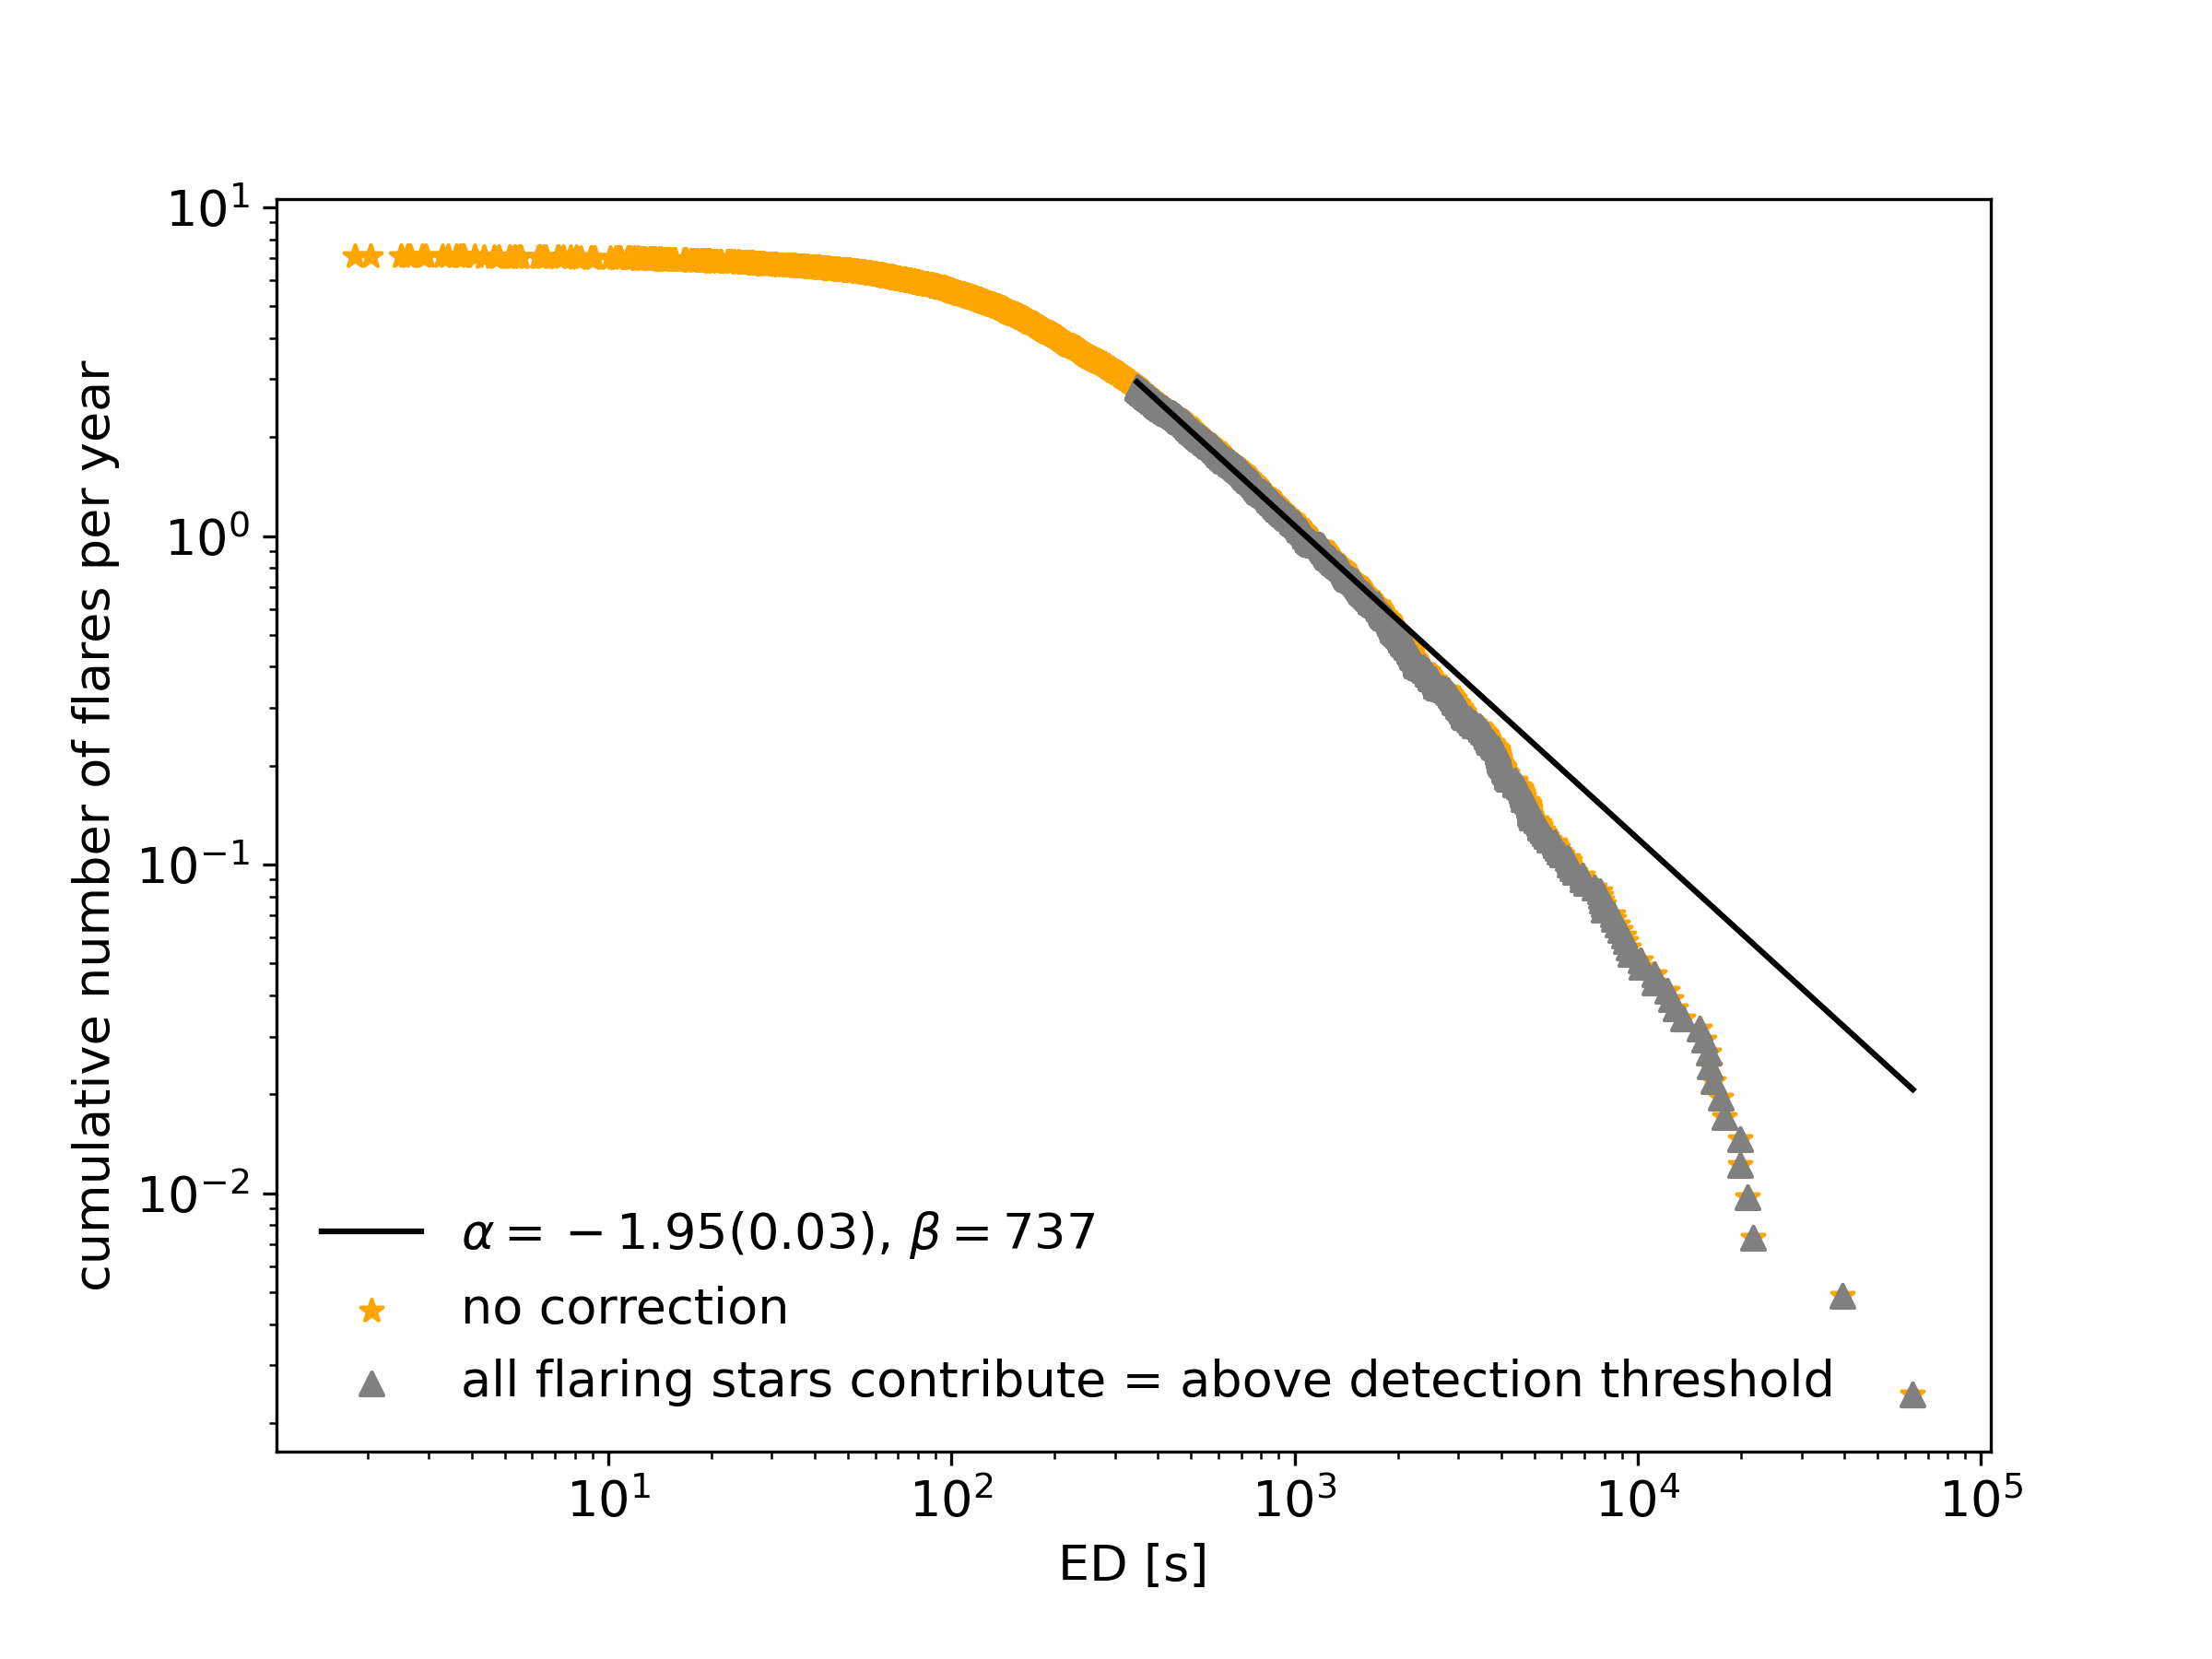
\includegraphics[width=0.49\hsize]{pics/FFDs/full_sample_ffd_ED.png}
    \hspace{.01cm}
    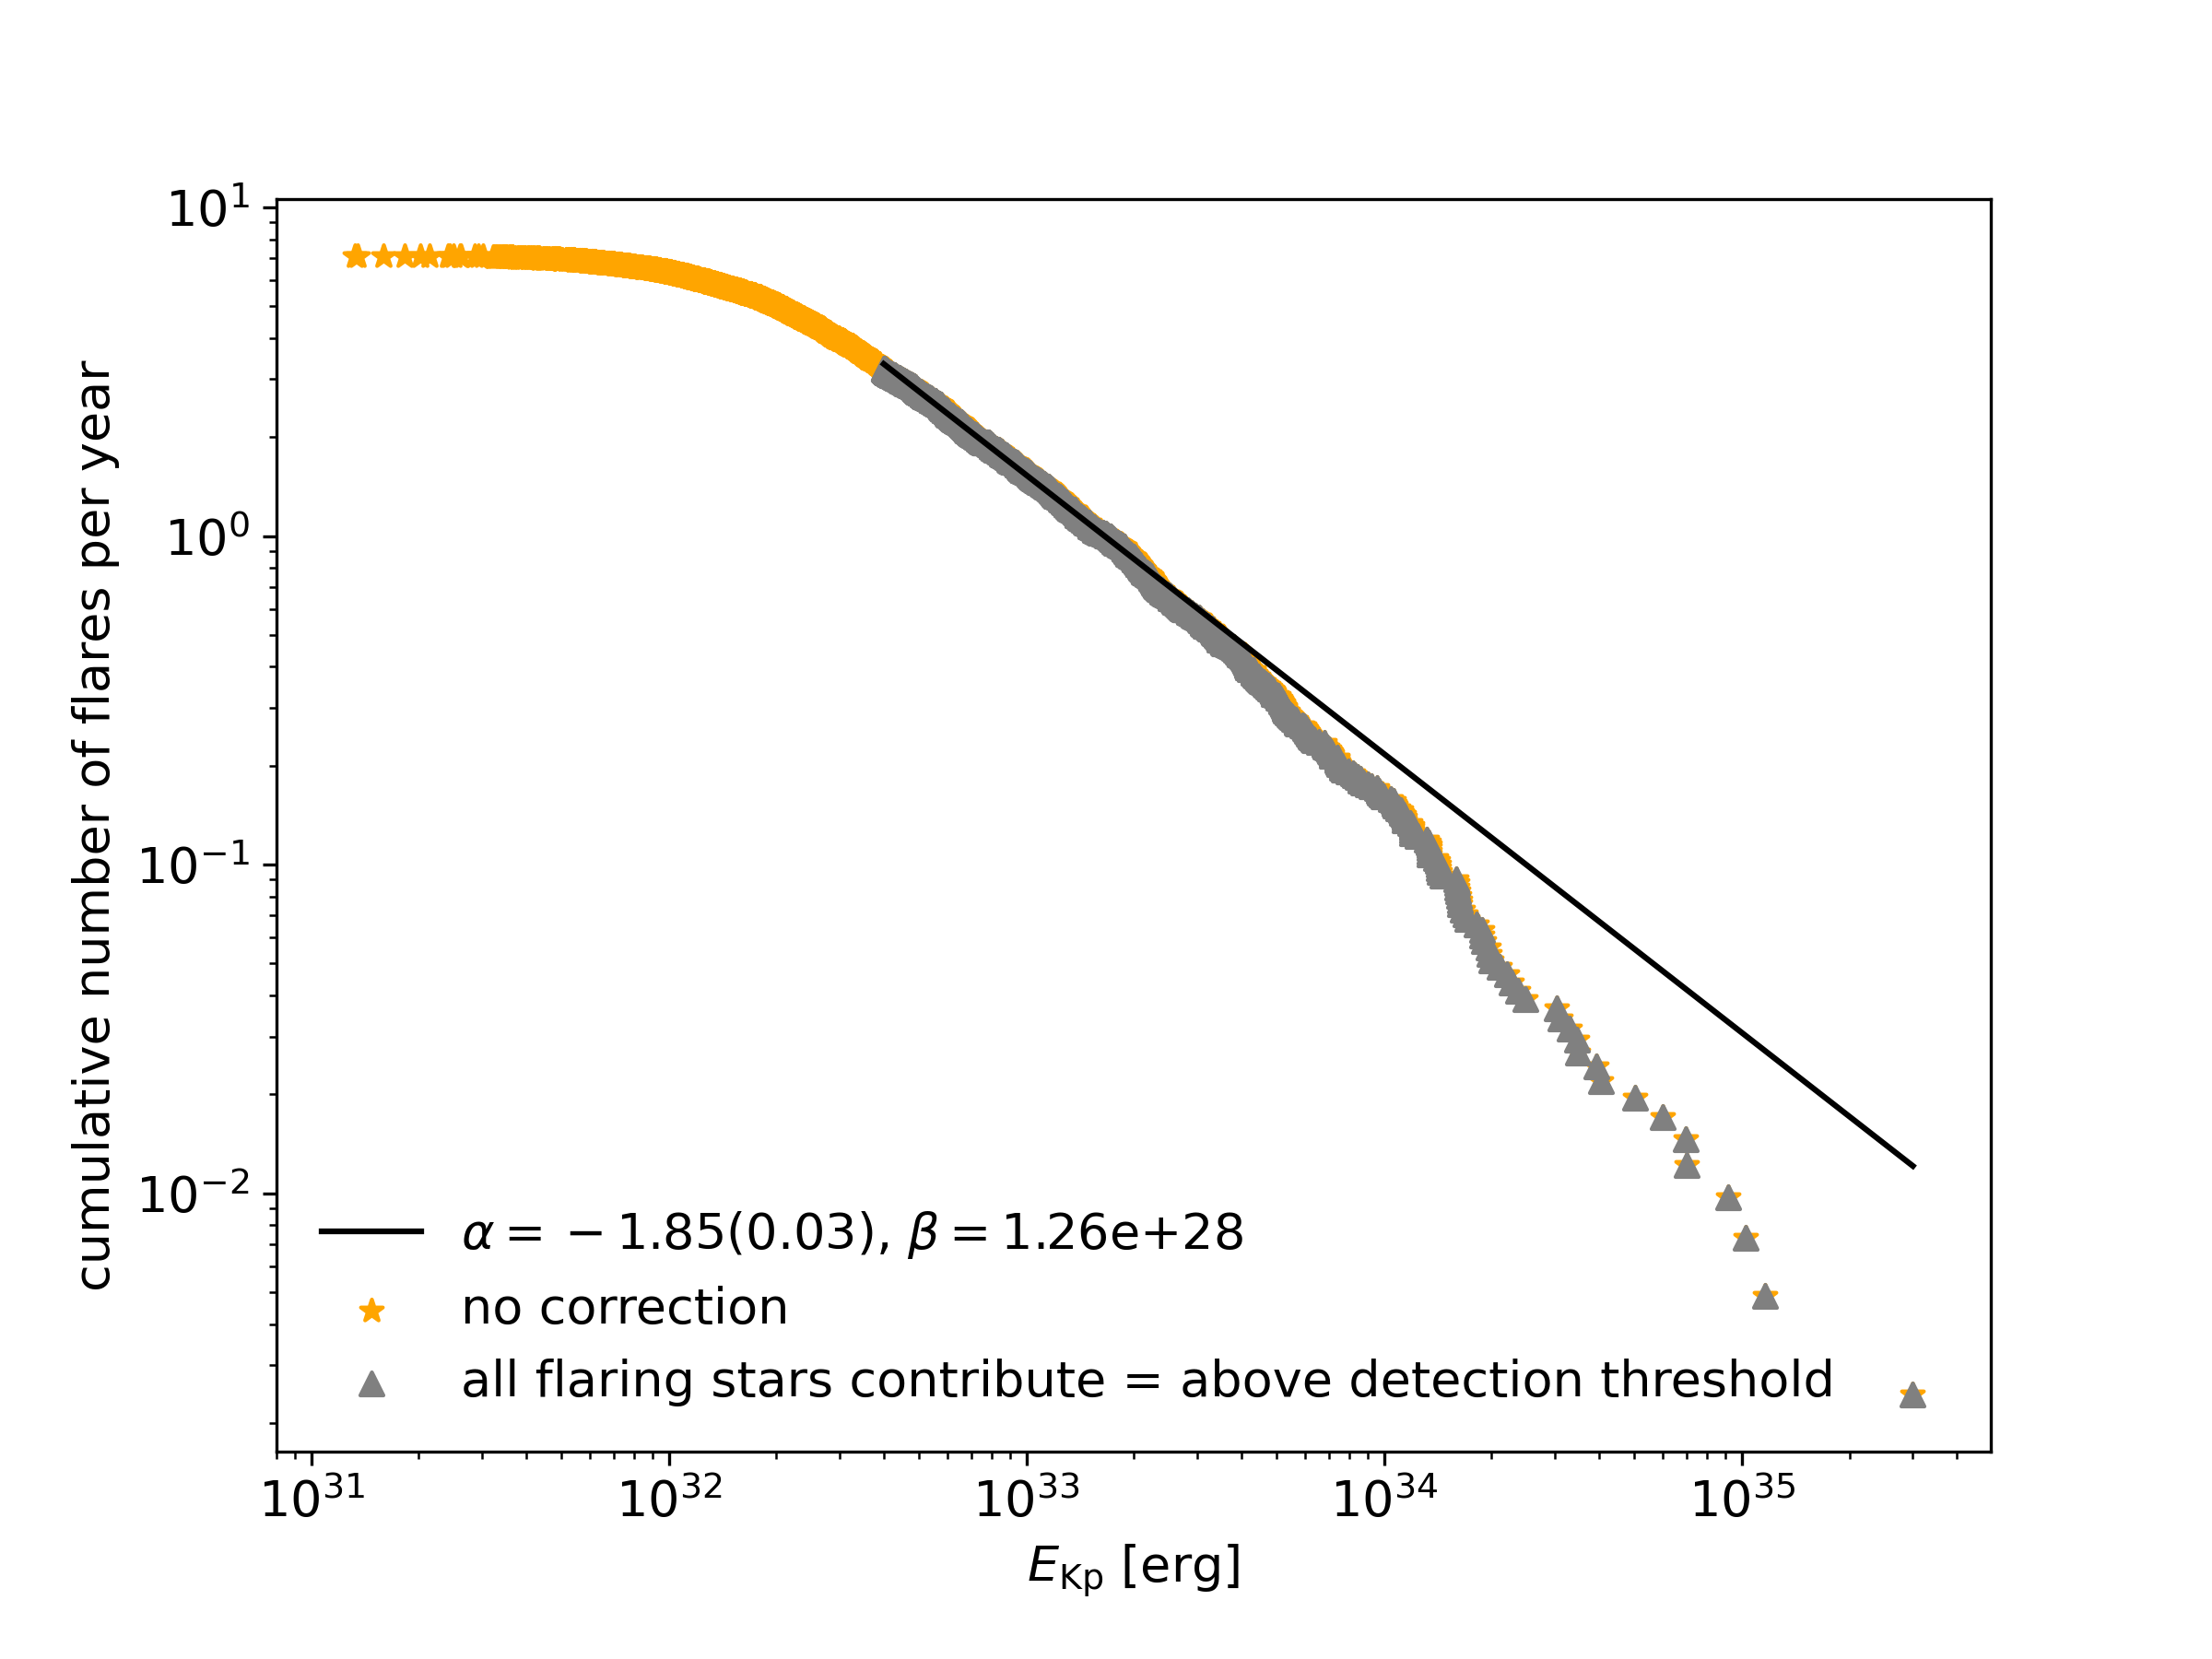
\includegraphics[width=0.49\hsize]{pics/FFDs/full_sample_ffd_energy.png}
    \caption{FFD (scatter) in $ED$ (left panel) and energy (right panel) and respective power law fit (black line) to the full sample of flare candidates.}          	
    \label{powerlawfit_full}
\end{figure*}

\begin{figure*}
    \centering
    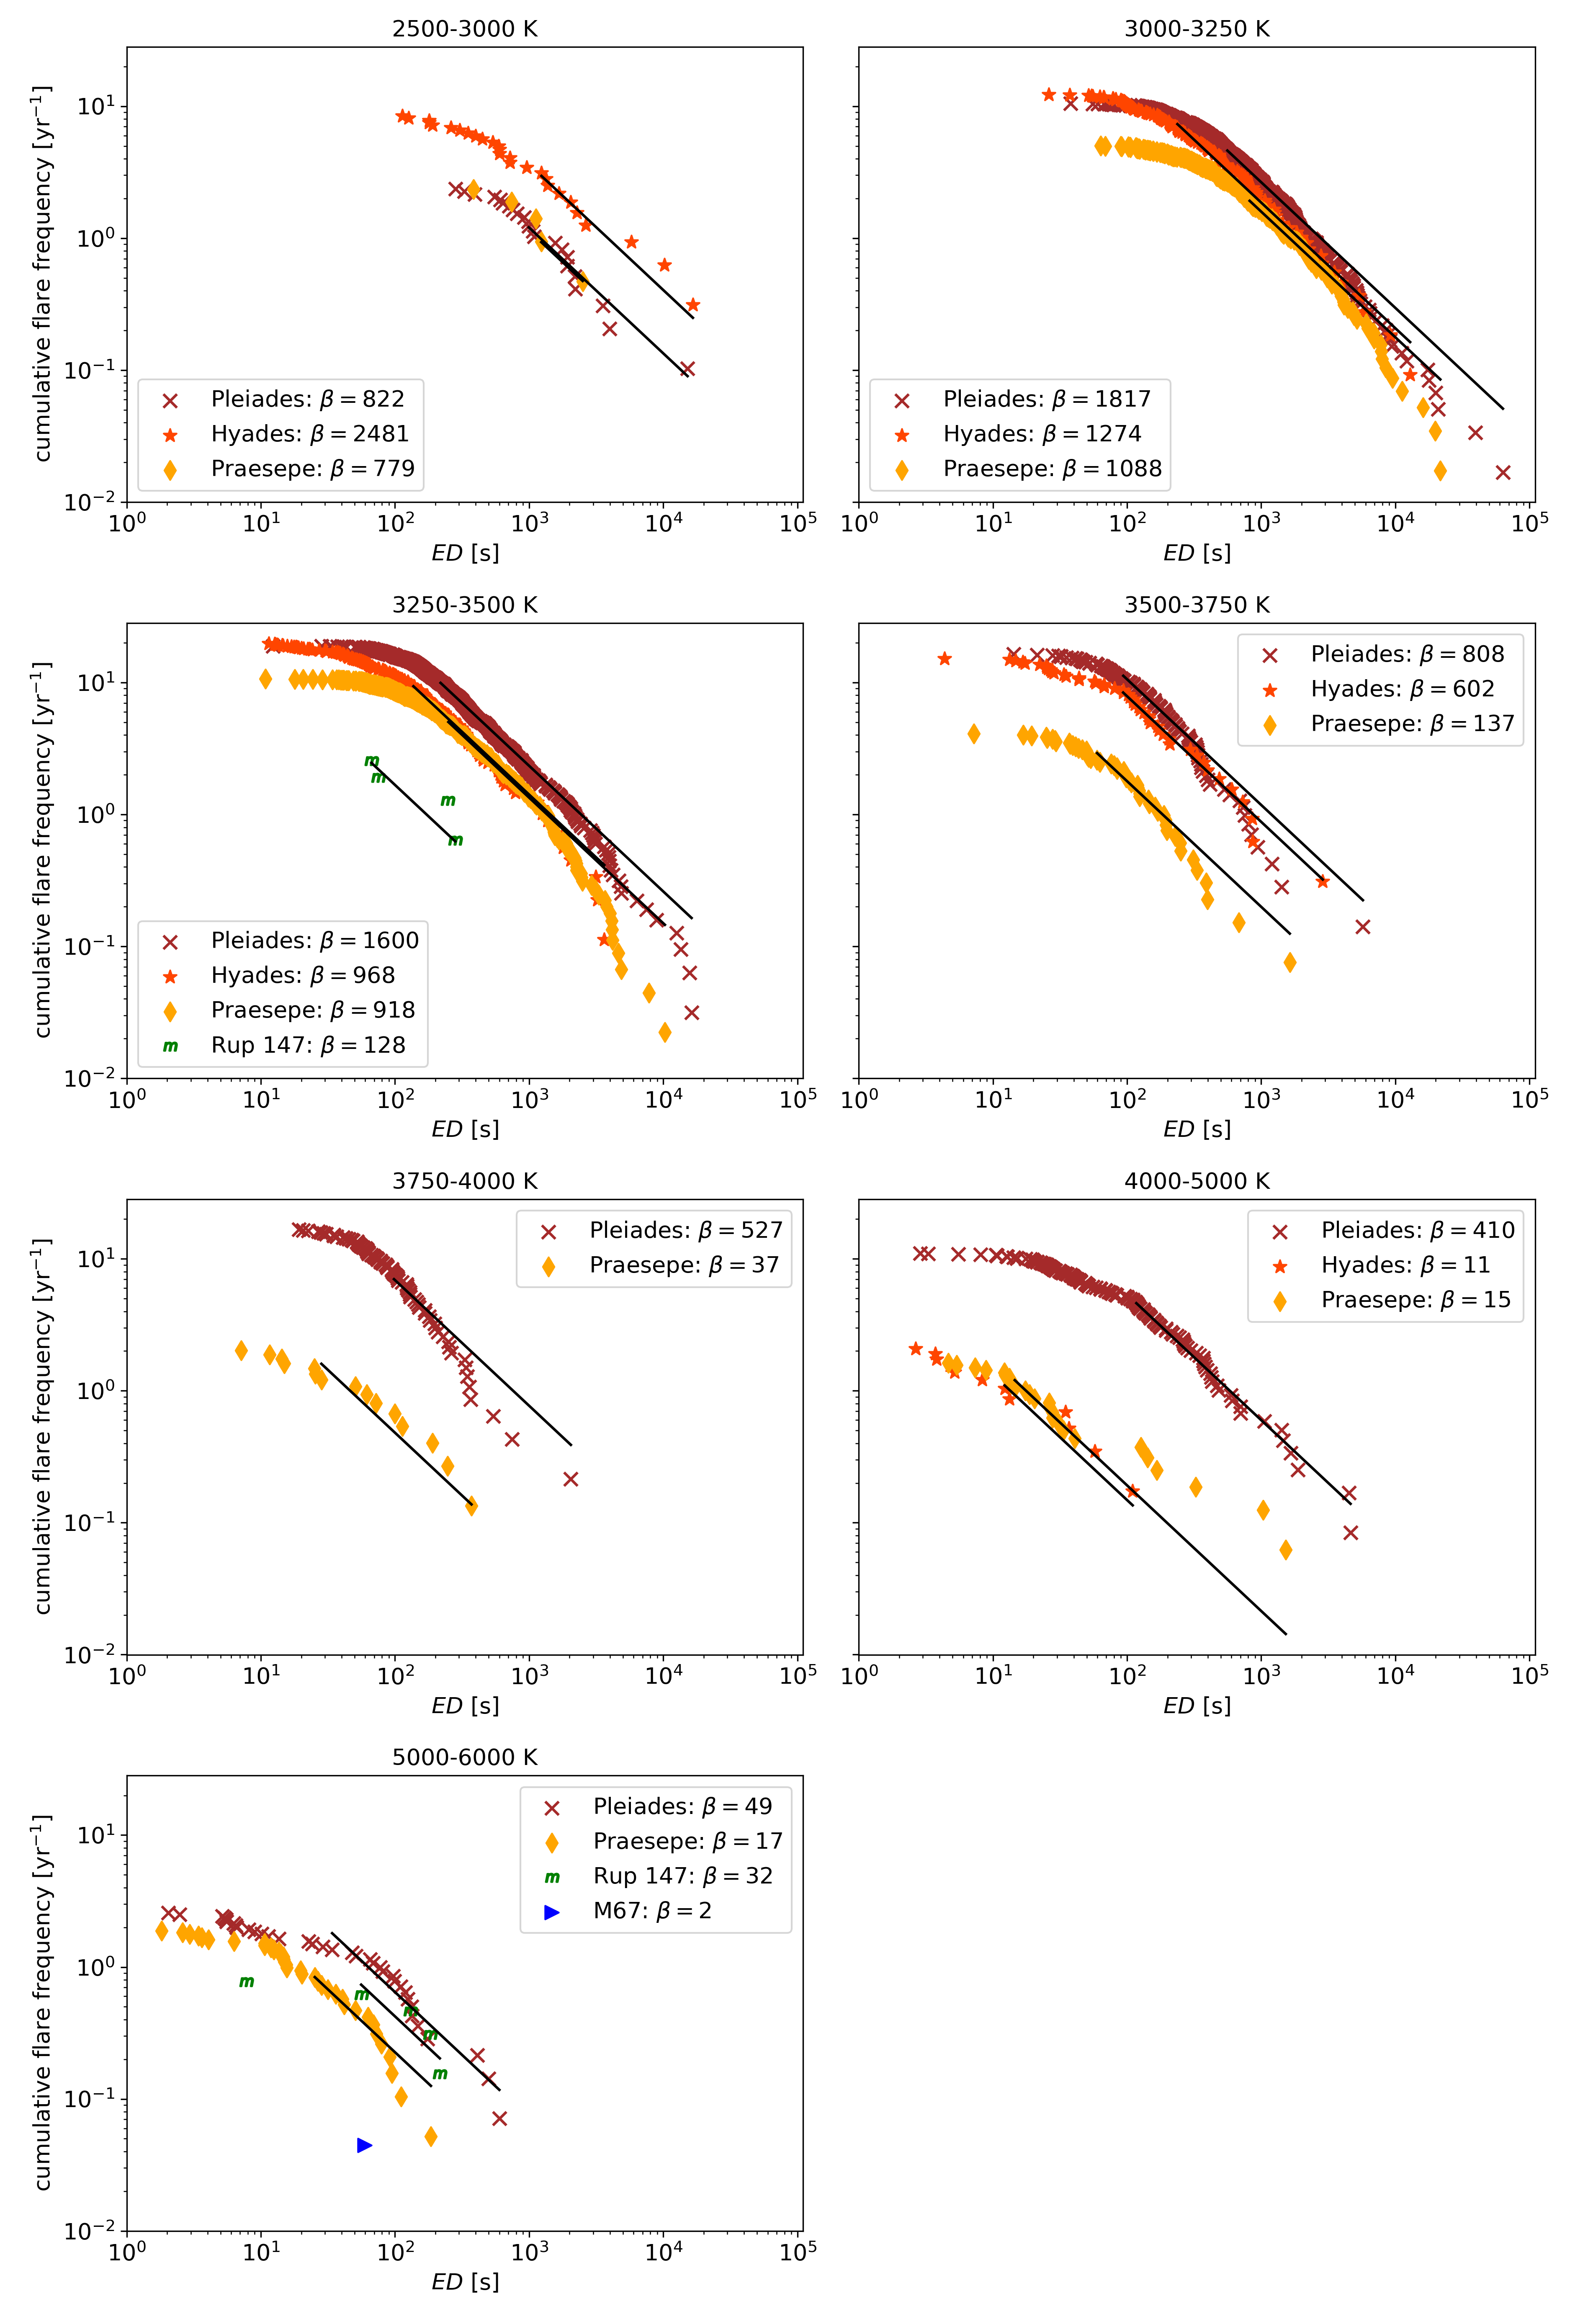
\includegraphics[width=16cm]{pics/FFDs/SpT_wise_sample_ffd_ED.png}
    \caption{FFDs (scatter) in $ED$ and respective power law fits with $\alpha=XXX$ (black lines).}          	\label{powerlawfits_s}
\end{figure*}

\begin{figure*}
    \centering
    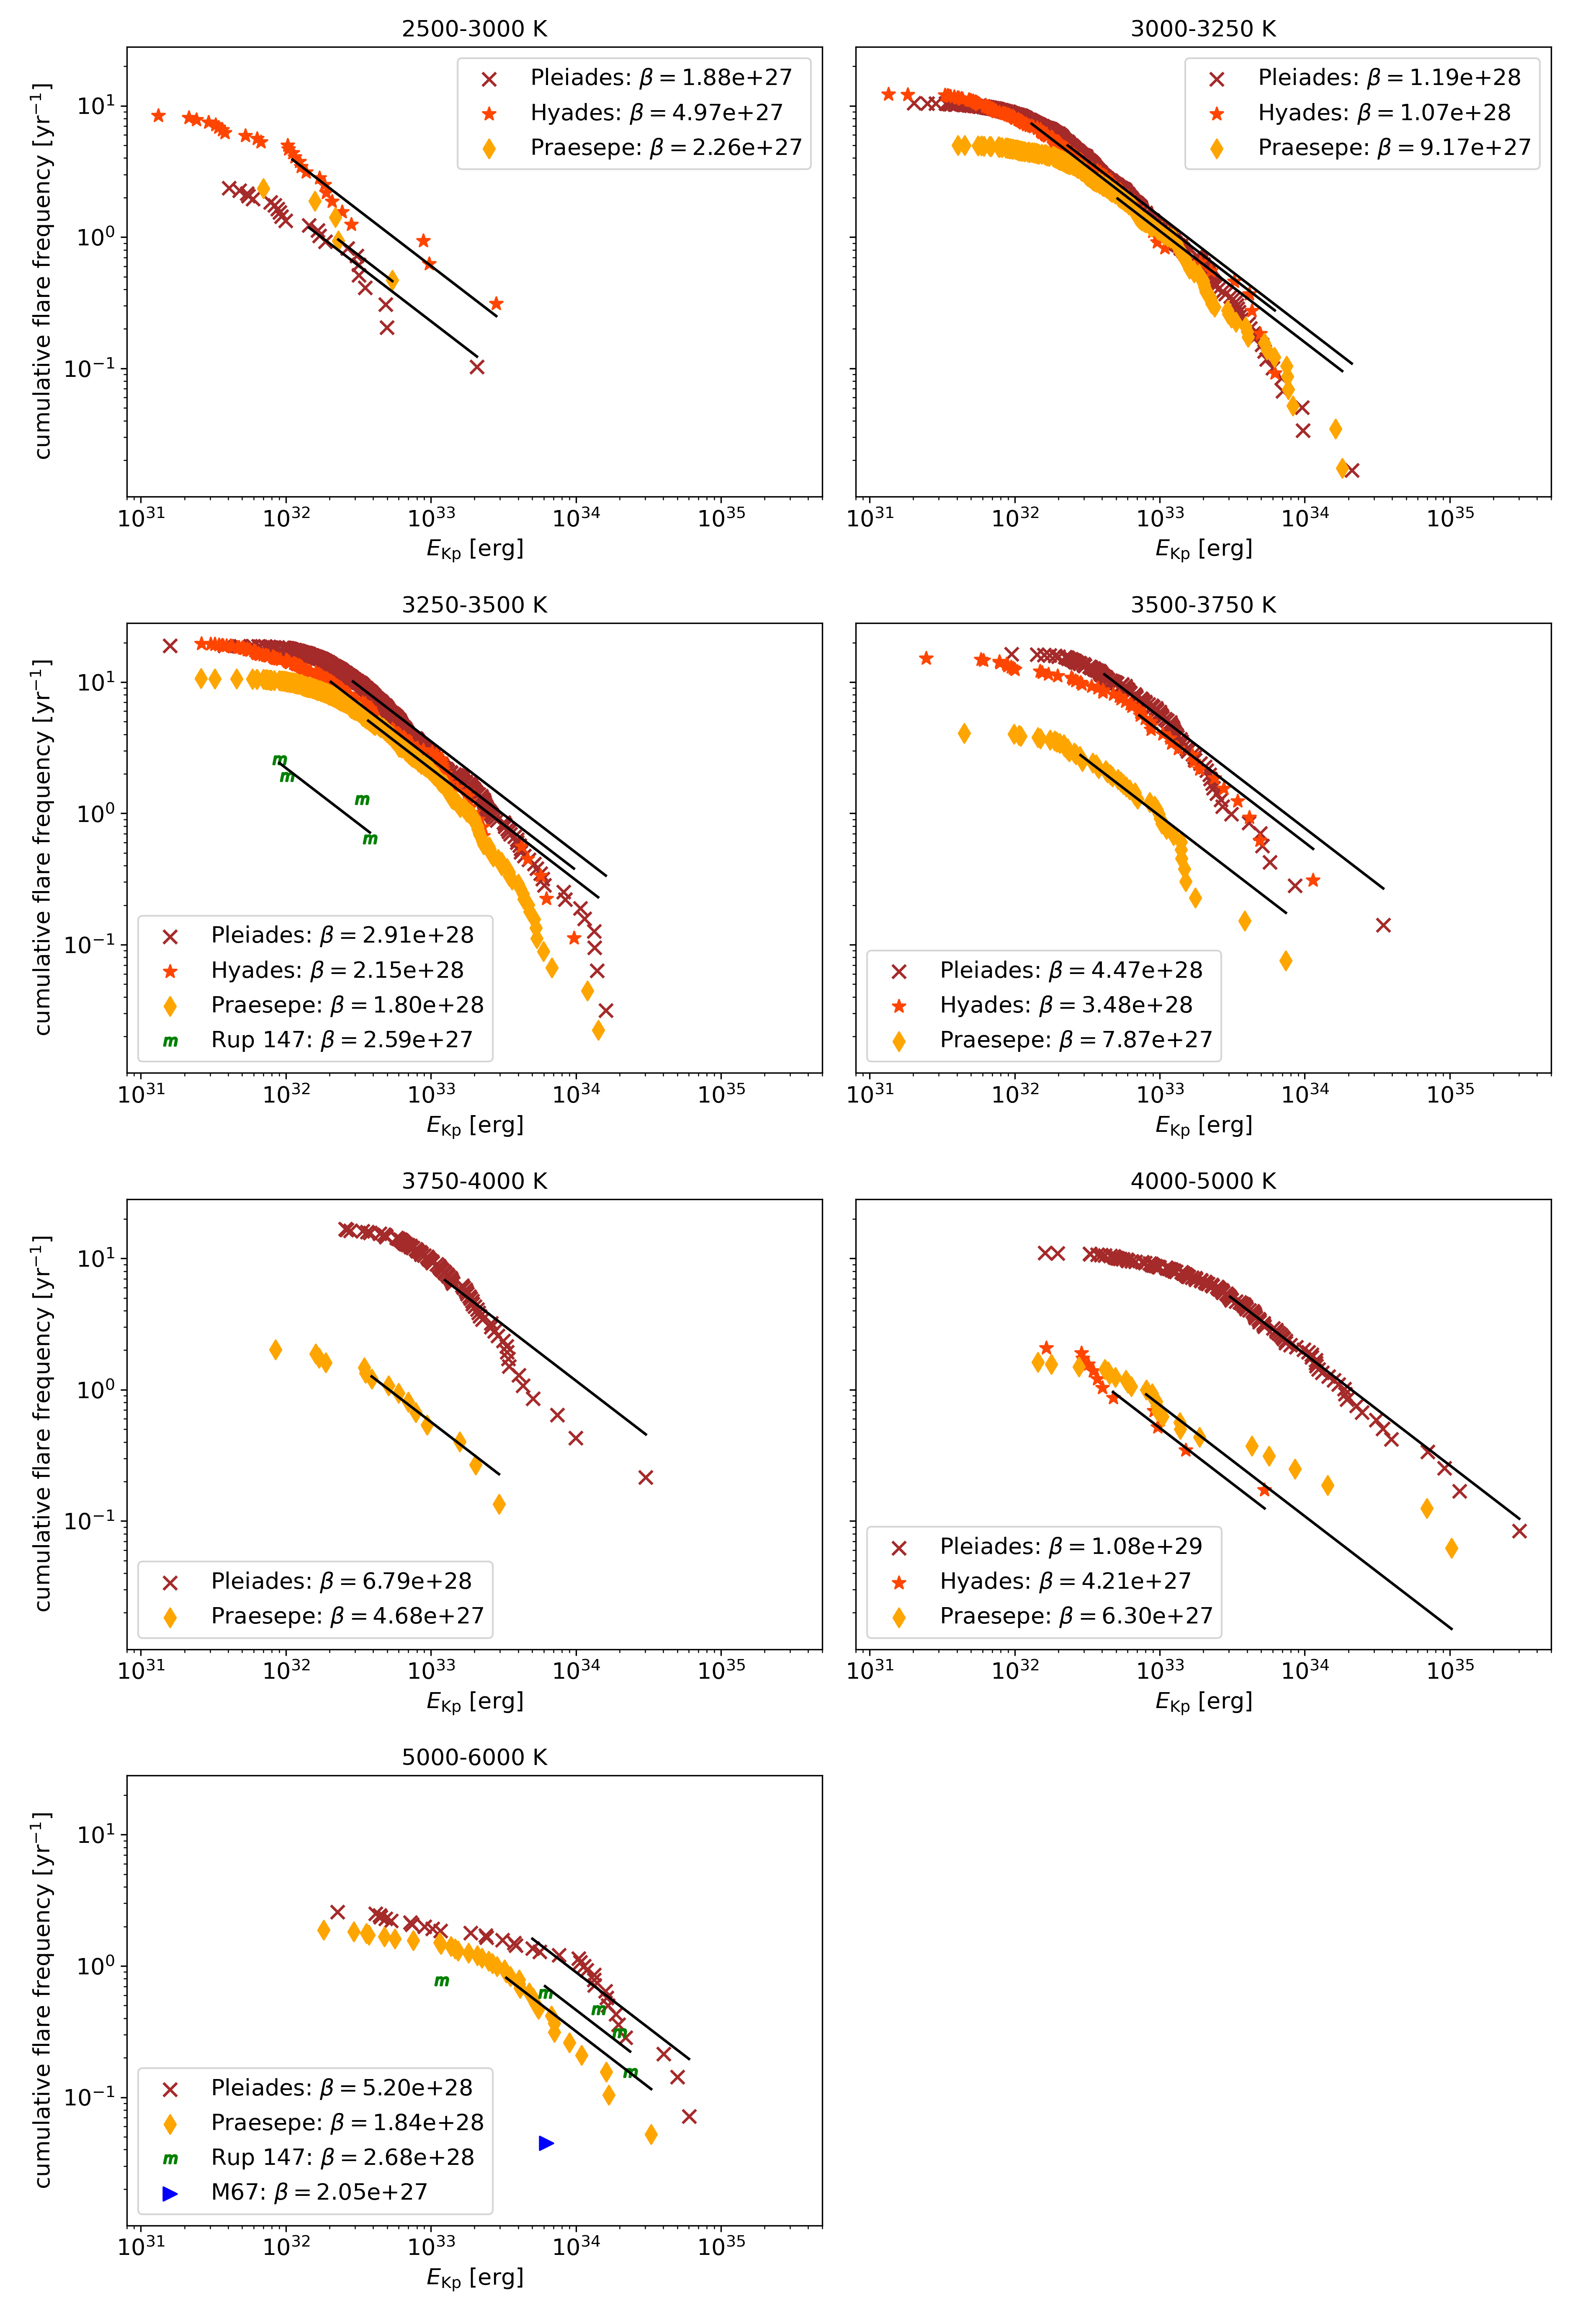
\includegraphics[width=16cm]{pics/FFDs/SpT_wise_sample_ffd_energy.png}
    \caption{FFDs (scatter) in energy and respective power law fits with $\alpha=XXX$ (black lines).}          	\label{powerlawfits_s}
\end{figure*}
%-------------------------------------------
% -- ALL POWERLAWS IN ERG
%-------------------------------------------

%         \caption{Power law fits to the FFDs of $E_\mathrm{Kp,flare}$ in Fig. \ref{ffds_teff_s}. See Fig. \ref{powerlawfits_s} for details.}
%-------------------------------------------
% BETA AND ALPHA IN ERG
%-------------------------------------------
%-------------------------------------------
%BETA AND ALPHA IN S
%-------------------------------------------

Fig. \ref{agemass_thresh} shows the $E_\mathrm{Kp,flare}$ and $ED$ detection thresholds, as defined by the recovery probability~(see Sec. \ref{recprob_edcor}). The thresholds in $ED$ reflect the noise level in the light curves.
%-------------------------------------------
\subsection{Flaring activity as a function of a age and $T_\mathrm{eff}$}
Flaring activity decays with age. Flaring fraction was observed to decline with galactic latitude for M dwarfs~\citep{hilton_dwarf_2010}Howard+2019. Short rotation periods and high magnetic activity measured in H$\alpha$ are strongly correlated~\citep{west_magneticrotationage_2015}. According to gyrochronology, fast rotation indicates young age~\citep{barnes_rotational_2003}, and slows down as the star ages. Here, we quantify how this decline unfolds for different spectral types. Except for the stars in our coolest temperature bin (M5.5-M8, 2\,500-3\,000 K), stellar flaring activity at a given age is always stronger for a cooler star. The exception is seen at cluster ages around 120 Myr.
\\
What creates the strong emission in white light? Extended flare loops, maybe~\citep{heinzel_flareloops_2018}
%-------------------------------------------
\subsection{M67 and Rup 147}
\begin{table}
\caption{Mass budget of flaring stars in M67 and Rup 147 within uncertainties on radius.}
\begin{tabular}{lcc}
\hline
 EPIC & median SpT &     binary \\
\hline
 211434440 &         K1 &    K2 + M5.5 \\
 219601739 &         G8 &      K1 + M6 \\
 219610232 &       K0.5 &    K2 + M5.5 \\
 219591752 &         M3 &  M3.5 + M3.5 \\
\hline
\end{tabular}
\end{table}
We found several flare candidates in stars that are members of M67 and Rup 147. However, all but the events that occurred on four stars were false postives (SSOs), or the stars were not single members. Flare candidates in these old clusters appeared on RS CVn binaries, cataclysmic binaries, Algol type binaries, spectroscopic and eclipsing bianries, and red giant stars. Excluding all these, we were left with one flare in M67 on a K1 dwarf. In Rup 147, we narrowed down the list to a flare on a G8 star in Rup 147, and four flares each on a K0.5 and an M3 star. For these stars, the multiplicity status is unknown. We found that the mass range of these stars as calculated from the uncertainties on their radii~\citep{eker2018} is large enough that the stars could in principle be binary stars with undetected mid-M dwarf companions.  
%-------------------------------------------
\subsection{Flaring Activity Indicators}
%-------------------------------------------
\paragraph{Flaring rates: $FR$ and flaring fraction}
We define $FR$ as the flare rate above detection thresholds on $E_\mathrm{Kp,flare}$ and $ED$ in each $T_\mathrm{eff}$ bin, respectively~(Figs. \ref{agemass_FR_flarefrac_erg} and \ref{agemass_FR_flarefrac_s}).
%-------------------------------------------
\paragraph{Flaring energy: $FA$ and $L_\mathrm{Kp,flare}$}
The energy released in flares was inferred using our derived stellar luminosities. It declines with age for every $T_\mathrm{eff}$ bin considered for both the total luminosity and relative to the quiescent flux~(Fig. \ref{agemass_FA_Lflare}).
\\
$L_\mathrm{Kp,flare}$ is the luminosity in flares in the Kepler band. We can relate this to the quiescent bolometric luminosity of the star when we define the fractional flare luminosity $FA$ as in \citetalias{ilin_flares_2019}:
\begin{align}
\label{FA}
FA&=\dfrac{1}{N}\displaystyle\sum_{i}^{N} FA_i = \dfrac{1}{N} \displaystyle\sum_{i}^{N} \dfrac{E_{\mathrm{Kp,flare,tot,}i}}{t_i\cdot L_{\mathrm{bol,*,}i}}
\end{align}
We determine $L_\mathrm{bol,*}$ from $R_*$ and $T_\mathrm{eff}$, as described in Sec.~\ref{TeffRL}. This is a meaningful measure of relative stellar activity as long as only the flux portion of the quiescent star in the Kepler band is roughly constant. It is therefore sensible to compare $FA$ values across ages, but not across $T_\mathrm{eff}$.
%\\
%\textit{We could test our results if we derived $FA$ from the bolometric correction suggested by \citet{davenport_flaresevolve_2019}. Would there be any difference?}
%-------------------------------------------
\paragraph{FFD}
Power law fit parameters to the FFDs~(Figs. \ref{ffds_teff_s} and \ref{ffds_teff_erg}) are sensitive to the low-energy cutoff, where most observations reside. The goodness of fit strongly depends on the sample size.
\\
Power law fit parameters derived using MLEs, as described in Sec. \ref{powerlawfits}, are mostly consistent with each other but often deviate from $\alpha=2$. A smaller sample size tends to create a flatter distribution~(Figs. \ref{powerlawfits_s} and \ref{powerlawfits_erg}). Truncation was not detected for FFDs with more than 50 flares~(Tables \ref{ergtable} and \ref{stable}) For these results, extrapolations outside of the observed energy range are clearly off. If we assume $\alpha \equiv 2$,  different distributions can be compared. For fixed $\alpha$, in the $ED$ domain, $\beta_2$ is the flare frequency at $ED=1\,\mathrm{s}$, and shows a trend in both $T_\mathrm{eff}$, and age (see Fig. \ref{agemass_alphabeta_s}). In the energy domain, the picture is less clear~(Fig. \ref{agemass_alphabeta_erg}).
\\
%~(called  $R1s$ in \citet{davenport_flaresevolve_2019})
%Maximum flare energy most likely determined by observation time as higher energies were observed before (cite Sarah and others, look up How big do flares get? in Loyd 2018)
%\\
\textit{Compare to other FFD values, e.g., from Ward's Evryscope survey, see table in Appendix, and maybe convert it to a plot}
Howard et al (2019) monitored superflares on cool stars with bolometric energies above $10^{33}$ erg and up to $10^{36}$erg. They find power law exponent values around $\sim 2$ resolved by spectral types. Similar values are found for individual flare stars~\citep{lurie_kepler_2015}.
\\
Howard+18, Loyd+18, Tilley+19 show that flares can erode exoplanetary atmospheres. If a flare is assumed to deposit its UV energy in an instant a single superflare can completely remove the ozone layer at the substellar point Loyd+18. Associated protons are safer way to ozone destruction if they are associated with reoccurring large flares Tilley+19
%-------------------------------------------
%-------------------------------------------
\begin{table*}
\caption{Summary of flaring $\beta$ of all clusters and $T_\mathrm{eff}$ bins in $E_\mathrm{Kp}$ and $ED$ distributions.}\label{powerlawtable_spt}
\centering
\begin{tabular}{lccccccccr}
\hline
          &         &                     $\beta_\mathrm{s}$ & $n_\mathrm{s}$ & $tr_\mathrm{s}$ & $pl_\mathrm{s}$ &                        $\beta_\mathrm{erg}$ & $n_\mathrm{erg}$ & $tr_\mathrm{erg}$ & $pl_\mathrm{erg}$ \\
\hline
2500-3000 & Hyades &     $2.48\left(0.1\right)\cdot 10^{3}$ &             27 &           False &            True &        $0.65\left(0.02\right)\cdot 10^{28}$ &               27 &             False &              True \\
          & Pleiades &    $0.82\left(0.03\right)\cdot 10^{3}$ &             23 &           False &            True &        $2.46\left(0.09\right)\cdot 10^{27}$ &               23 &             False &              True \\
          & Praesepe &  $0.777\left(0.024\right)\cdot 10^{3}$ &              5 &           False &            True &      $2.968\left(0.093\right)\cdot 10^{27}$ &                5 &             False &              True \\
3000-3250 & Hyades &    $1.27\left(0.04\right)\cdot 10^{3}$ &            133 &           False &            True &      $1.401\left(0.038\right)\cdot 10^{28}$ &              133 &             False &              True \\
          & Pleiades &  $1.814\left(0.055\right)\cdot 10^{3}$ &            623 &           False &            True &      $1.559\left(0.042\right)\cdot 10^{28}$ &              623 &              True &              True \\
          & Praesepe &  $1.086\left(0.033\right)\cdot 10^{3}$ &            289 &            True &            True &      $1.205\left(0.033\right)\cdot 10^{28}$ &              289 &              True &              True \\
3250-3500 & Hyades &   $0.966\left(0.03\right)\cdot 10^{3}$ &            175 &           False &            True &      $2.812\left(0.076\right)\cdot 10^{28}$ &              175 &             False &              True \\
          & Pleiades &  $1.597\left(0.049\right)\cdot 10^{3}$ &            598 &            True &            True &       $0.382\left(0.01\right)\cdot 10^{29}$ &              598 &              True &              True \\
          & Praesepe &  $0.917\left(0.028\right)\cdot 10^{3}$ &            477 &            True &            True &       $2.36\left(0.064\right)\cdot 10^{28}$ &              477 &              True &             False \\
          & Rup 147 &    $1.28\left(0.12\right)\cdot 10^{2}$ &              4 &           False &            True &        $0.34\left(0.03\right)\cdot 10^{28}$ &                4 &             False &              True \\
3500-3750 & Hyades &     $0.6\left(0.02\right)\cdot 10^{3}$ &             49 &           False &            True &      $0.458\left(0.014\right)\cdot 10^{29}$ &               49 &             False &              True \\
          & Pleiades &  $0.807\left(0.025\right)\cdot 10^{3}$ &            116 &           False &            True &      $0.588\left(0.016\right)\cdot 10^{29}$ &              116 &             False &              True \\
          & Praesepe &    $1.36\left(0.05\right)\cdot 10^{2}$ &             54 &           False &            True &      $1.032\left(0.031\right)\cdot 10^{28}$ &               54 &             False &              True \\
3750-4000 & Pleiades &    $0.53\left(0.02\right)\cdot 10^{3}$ &             78 &           False &            True &        $0.89\left(0.03\right)\cdot 10^{29}$ &               78 &             False &             False \\
          & Praesepe &    $0.37\left(0.08\right)\cdot 10^{2}$ &             15 &           False &            True &        $0.61\left(0.02\right)\cdot 10^{28}$ &               15 &             False &              True \\
4000-5000 & Hyades &    $1.13\left(0.11\right)\cdot 10^{1}$ &             12 &           False &            True &        $0.55\left(0.06\right)\cdot 10^{28}$ &               12 &             False &              True \\
          & Pleiades &   $0.41\left(0.013\right)\cdot 10^{3}$ &            131 &           False &            True &      $1.434\left(0.039\right)\cdot 10^{29}$ &              131 &             False &              True \\
          & Praesepe &    $1.46\left(0.07\right)\cdot 10^{1}$ &             26 &           False &            True &        $0.83\left(0.03\right)\cdot 10^{28}$ &               26 &             False &              True \\
5000-6000 & M67 &    $2.19\left(0.31\right)\cdot 10^{0}$ &              1 &            True &           False &  $2.70328\left(0.00027\right)\cdot 10^{27}$ &                1 &              True &             False \\
          & Pleiades &    $0.49\left(0.05\right)\cdot 10^{2}$ &             36 &           False &            True &        $0.69\left(0.04\right)\cdot 10^{29}$ &               36 &             False &              True \\
          & Praesepe &    $1.73\left(0.06\right)\cdot 10^{1}$ &             36 &           False &            True &        $2.44\left(0.09\right)\cdot 10^{28}$ &               36 &             False &              True \\
          & Rup 147 &    $0.32\left(0.08\right)\cdot 10^{2}$ &              5 &           False &            True &        $0.36\left(0.05\right)\cdot 10^{29}$ &                5 &             False &              True \\
\hline

\end{tabular}

\end{table*}
\begin{table}
\caption{Summary of FFD parameters and power law fits to the full sample of all clusters in $E_\mathrm{Kp}$ and $ED$ space.}\label{powerlawtable_fullsample}
\centering
\begin{tabular}{lccr}
\hline\hline
  &        $ED$ &      $E_\mathrm{Kp}$ \\
\hline
$\alpha$            &  1.95(0.03) &           1.85(0.03) \\
$\beta$ [yr$^{-1}$] &     785(24) &  1.75(0.05)$10^{28}$ \\
$n_\mathrm{tot}$    &        2913 &                 2913 \\
$n_\mathrm{fit}$    &        1166 &                 1336 \\
$tr$                &        True &                 True \\
$pl$                &       False &                False \\
\hline

\end{tabular}

\end{table}
%\begin{sidewaystable*}
%\caption{Summary of activity parameters of all clusters and $T_\mathrm{eff}$ bins in equivalent duration distributions.}\label{stable}
%\centering
%\tiny
%\begin{tabular}{lrrrrllllllllrrr}
\toprule
  cluster &  $T_\mathrm{min} [\mathrm{K}]$ &  $T_\mathrm{max} [\mathrm{K}]$ &  $n_*$ &  $n_\mathrm{flares}$ &               age [Myr] &          [Fe/H] & $ED$$_\mathrm{min}\;[$s$]$ & $\alpha_\mathrm{B}$ & $\alpha_\mathrm{MK}$ & $\beta_2\;[\mathrm{yr}^{-1}]$ & $\beta_\mathrm{B}\;[\mathrm{yr}^{-1}]$ & $\beta_\mathrm{MK}\;[\mathrm{yr}^{-1}]$ &  $tr_2$ &  $tr_\mathrm{B}$ &  $tr_\mathrm{MK}$ \\
\midrule
 Pleiades &                           4000 &                           4999 &     87 &                  110 &     $125\pm _{25}^{25}$ &  $-0.02\pm0.03$ &        $2.3 \cdot 10^{1}$ &     $1.68$$\pm0.07$ &        $1.68\pm0.07$ &               $175.40\pm3.06$ &                         $26.23\pm1.80$ &                          $26.08\pm1.74$ &       0 &                0 &                 0 \\
 Pleiades &                           3000 &                           3249 &    353 &                  129 &     $125\pm _{25}^{25}$ &  $-0.02\pm0.03$ &        $9.1 \cdot 10^{2}$ &     $2.26$$\pm0.12$ &        $2.24\pm0.12$ &              $1663.97\pm8.43$ &                   $16801.52\pm1988.56$ &                    $14323.95\pm1675.01$ &       0 &                0 &                 0 \\
 Pleiades &                           3250 &                           3499 &    168 &                  185 &     $125\pm _{25}^{25}$ &  $-0.02\pm0.03$ &        $2.2 \cdot 10^{2}$ &     $2.03$$\pm0.09$ &        $2.02\pm0.09$ &              $1250.16\pm3.32$ &                     $1524.74\pm130.65$ &                      $1437.66\pm122.52$ &       0 &                0 &                 0 \\
 Pleiades &                           2500 &                           2999 &     63 &                   28 &     $125\pm _{25}^{25}$ &  $-0.02\pm0.03$ &          $2 \cdot 10^{2}$ &     $1.40$$\pm0.32$ &        $1.38\pm0.26$ &              $732.64\pm89.39$ &                          $3.07\pm0.97$ &                           $2.55\pm0.68$ &       0 &                1 &                 1 \\
 Pleiades &                           3750 &                           3999 &     52 &                   61 &     $125\pm _{25}^{25}$ &  $-0.02\pm0.03$ &        $4.6 \cdot 10^{1}$ &     $1.86$$\pm0.12$ &        $1.84\pm0.11$ &               $337.15\pm3.77$ &                       $133.53\pm15.57$ &                        $118.85\pm13.38$ &       0 &                0 &                 0 \\
 Pleiades &                           5000 &                           5999 &     53 &                   14 &     $125\pm _{25}^{25}$ &  $-0.02\pm0.03$ &                      $4.9$ &     $1.27$$\pm0.25$ &        $1.32\pm0.17$ &                 $9.24\pm1.16$ &                          $0.13\pm0.03$ &                           $0.20\pm0.04$ &       0 &                1 &                 1 \\
 Pleiades &                           3500 &                           3749 &     50 &                   47 &     $125\pm _{25}^{25}$ &  $-0.02\pm0.03$ &        $1.6 \cdot 10^{2}$ &     $1.88$$\pm0.11$ &        $1.84\pm0.11$ &               $838.25\pm8.01$ &                       $338.29\pm38.96$ &                        $256.41\pm28.27$ &       0 &                0 &                 0 \\
      M35 &                           4000 &                           4999 &    221 &                    7 &     $149\pm _{13}^{13}$ &  $-0.21\pm0.06$ &        $5.2 \cdot 10^{2}$ &                   - &        $1.34\pm0.76$ &              $202.70\pm21.23$ &                                      - &                           $0.26\pm0.20$ &       1 &                0 &                 1 \\
  Rup 147 &                           5000 &                           5999 &     39 &                    7 &  $2301\pm _{257}^{380}$ &   $0.08\pm0.04$ &                      $4.0$ &                   - &        $1.95\pm0.30$ &                 $3.07\pm0.21$ &                                      - &                           $2.58\pm0.79$ &       0 &                0 &                 0 \\
   Hyades &                           4000 &                           4999 &     32 &                   22 &     $665\pm _{70}^{70}$ &   $0.13\pm0.01$ &                      $4.4$ &                   - &        $1.13\pm0.25$ &                $30.87\pm8.30$ &                                      - &                           $0.05\pm0.01$ &       0 &                0 &                 1 \\
   Hyades &                           3000 &                           3249 &     56 &                   14 &     $665\pm _{70}^{70}$ &   $0.13\pm0.01$ &        $9.8 \cdot 10^{2}$ &     $1.87$$\pm0.60$ &        $1.78\pm0.48$ &             $1037.31\pm28.99$ &                      $316.11\pm191.27$ &                        $132.35\pm63.88$ &       0 &                1 &                 1 \\
   Hyades &                           3250 &                           3499 &     42 &                   20 &     $665\pm _{70}^{70}$ &   $0.13\pm0.01$ &        $5.5 \cdot 10^{2}$ &     $1.82$$\pm0.37$ &        $1.77\pm0.30$ &             $1281.92\pm18.75$ &                       $264.94\pm97.28$ &                        $156.31\pm46.78$ &       0 &                0 &                 1 \\
   Hyades &                           3750 &                           3999 &      5 &                   21 &     $665\pm _{70}^{70}$ &   $0.13\pm0.01$ &                      $3.9$ &     $1.46$$\pm0.29$ &        $1.49\pm0.27$ &               $157.65\pm8.25$ &                          $8.37\pm2.48$ &                          $10.09\pm2.71$ &       0 &                1 &                 1 \\
   Hyades &                           5000 &                           5999 &     11 &                    8 &     $665\pm _{70}^{70}$ &   $0.13\pm0.01$ &        $2.4 \cdot 10^{1}$ &                   - &        $1.06\pm0.28$ &              $182.82\pm18.30$ &                                      - &                           $0.01\pm0.00$ &       1 &                0 &                 1 \\
   Hyades &                           3500 &                           3749 &     14 &                   30 &     $665\pm _{70}^{70}$ &   $0.13\pm0.01$ &                      $6.5$ &                   - &        $1.14\pm0.16$ &              $172.86\pm33.54$ &                                      - &                           $0.18\pm0.03$ &       0 &                0 &                 1 \\
\bottomrule
\end{tabular}

%\end{sidewaystable*}
%-------------------------------------------
%-------------------------------------------
% \subsection{Trends with Multiplicity}
% \label{results_multiplicity}
% Multiplicity rates for low-mass stars decrease from about 50\% for F type stars~\citep{raghavan_multiplicity_2010} to 22\% for L and T dwarfs~\citep{duchene_multiplicity_2013}, with M dwarf having somewhat higher multiplicity rates at about 27\% (Winters+2019).
% \\
% A discussion is only possible for OCs with binarity info. Is it only boolean info or do we also have a mass ratio?\\
% Give histograms (\#LCs in an activity bin) $-$ if intrinsic variability is not too strong, we may see a binary shoulder of even second peak. We expect a spread at least due to the different mass ratios. Mass ratio distribution is non-trivial in itself, few chances we can resolve that on top of intrinsic activity spread but we can try to do a histogram with binaries only at some stage.
% \\
% Kouwenhoven et al. (2009):  $30-40\,\%$ of M dwarfs are members of a binary system. For late M dwarfs and brown dwarfs this drops to $10 - 30\,\%$.
%ChangQing Luo+19 inspect an interacting M dwarf (M1+M3.5, BX Tri) eclipsing binary that exhibits superflares and strong hydrogen emission (semi-detached system, references to other observations of BX Tri)
\section{Discussion}
\subsection{Consistency with other studies}
EvryFlare, mass-dependence,
\subsection{Flaring and rotation}
More energetic flares can be expected from faster rotating stars~\citep{candelaresi_superflare_2014, doorsselaere_stellar_2017, yang_flaring_2017}. Findings that flares with intermediate Rossby number appear to flare more than fast and slow rotators~\citep{mondrik_flarerotation_2019} could not be reproduced here or in the EvryFlare survey~\citep{howard_evryflare2arxiv_2019}. If enhanced flaring can be interpreted as an increase in the stellar angular momentum loss rate flaring activity can be used to inform the cause of variation in the spin-down efficiency. An example of such variations is the apparent temporary stalling of spin-down seen in K dwarfs in NGC 6811~(Curtis+2019). The authors favored a scenario in which the stellar core transfers momentum onto the envelope but did not rule out the possibility of a decreased magnetic braking efficiency. In the latter scenario, these stars should flare less. %What do Cecilia's models say about the change in MF regime in these stars?
\\
We used rotation periods derived from K2 light curves for the Pleiades~\citep{rebull_pleiadesrot_2016}, the Hyades~\citep{douglas_hyadesrot_2016}, and Praesepe~\citep{rebull_praesepe_2017}, to illuminate the rotation-flaring relation at fixed ages. In the Pleiades, most flaring stars are found on the fast rotator branch at or below one day, and flaring activity peaks in this regime. For Praesepe, flaring rates aappear t ..[...]. In the Hyades, all of the 11 stars with rotation periods that overlapped with our sample were found flaring, but the number were too low to provide statistical insight. For Rup 147, M35 and M67, no rotation rates were available at the time.
 \subsection{M37}
Comparing our results to a similar study of photometric flares in M37~\citep{chang_photometric_2015} we find the results somewhat discrepant. M37 is 300-600 Myr old and appears less active than Praesepe and Hyades in individual Teff bins, which are of coeval or older. We attribute the difference to the loose membership requirement of $pmem \geq 0.2$ in~\cite{chang_photometric_2015} as compared to our stricter cuts at 0.8. We expect the M37 to be contaminated with field stars that systematically reduce the flaring rates. Applying our own restriction the M37 sample~\citep{chang_photometric_2015_data} leaves very few flares that hamper a statistical description of their distributions.
\subsection{Division at 3000 K}
The lowest $T_\mathrm{eff}$ bin at Pleiades age in our sample reflects the division between fully convective stars and those with a radiative core~\citep{reid_new_2005}. At this age, the coolest dwarfs may still be accreting angular momentum on the PMS, instead of spinning down on the MS. We suggest that a regime change occurs around 120 Myr for stars with $T_\mathrm{eff}=2500-3250$ K.
\\
Below 3000 K, an analysis of 66 ZDI maps show that magnetic field configurations can be strong and dipolar or weak and multipolar~\citep{morin_m4magneticfields_2008, see_zdispindown_2017}. If these stars can be distinguished by age, this should be reflected in our age-resolved flaring activity. If the difference is not a function of age, we should see a similar bimodal distribution of very inactive and very active stars in the lowest mass bins. If the difference between the two configurations is a function of age, we should only see one type of stars with correspondingly similar behaviour in these $T_\mathrm{eff}$ bins.
\\
The lowest mass bin appears underactive compared to the rest of the flaring-age-$T_\mathrm{eff}$ relation in the $ED$ domain. Physical explanations for this peculiarity include:
A different magnetic structure
A truncation of the power law that reflects the maximum $ED$ an active region can produce on these stars.
\\
\citet{west_magneticrotationage_2015} found that all M1-M4 dwarfs with rotation periods shorter than 26 days, and all M5-M8 dwarfs with periods shorter than 86 days show H$\alpha$ emission, indicating their magnetic activity.
\\
Assuming a typical binary fraction for early and mid M dwarfs~\citep{fischer_multiplicity_1992}, we can expect some of the flares on stars at $T_\mathrm{eff}>3000$ K to belong to unresolved binary companions with $T_\mathrm{eff}<3000$ K. A misattributed flare on an early M dwarf then will be assigned a too small $ED$, but still a correct $E_\mathrm{Kp, flare}$ because the count ratios are equal to the $L_\mathrm{Kp}$ ratios.
\subsection{Consistency of Hyades' and Praesepe's results}
HRDs constructed in \citet{gaia_dr2_2018_hrd} indicate only slightly older ages for Hyades and Praesepe. We expect our results to reflect this similarity.
\\
\textit{Are the samples comparable? Membership determination may differ.
Can we frame this as a statistical test, i.e. answer the question: What is the probability that the activity distributions for both clusters were drawn from the same underlying distribution for a given age and mass bin?}
\\
Metallicity is controlled for ([Fe/H](Praesepe)\,$=0.16$, [Fe/H](Hyades)\,$=0.13$, Netopil et al. 2016).
\subsection{Consistency of Pleiades and M35 results}
M35 is has subsolar metallicity, while Pleiades are rougly solar.
% \subsection{Can we use flaring activity as a pointer to unresolved binarity?}
% See Section \ref{results_multiplicity}.
\subsection{Jim's section(s)}
Flaring activity function of mass and age $-$ a gyrochronology analog?
\\
Results in the context of \citet{davenport_flaresevolve_2019}:
How well does the model fit if we have isochronal and not rotational ages for our stars?
\\
\citet{davenport_flaresevolve_2019} note a sample bias towards more active stars. Their models overpredicts the superflaring rate of the average Sun-like sample from~\citet{shibayama_2013} and more resembles the rate for their most active sub-sample. \textit{Do we see the same effect in our OC sample? We should not. Or cluster memberships depend on activity.}
\subsection{Universality of $\alpha$}
Takin into account uncertainties and systematic errors resulting power law fitting methods, the power law exponent $\alpha\sim 2$ appears to be the same for all studies on flare statistics so far, irrespective of spectral type. A noteable exception are A stars in Kepler that follow a power law with $\alpha\sim 1$ that may indicate a different physical process~\citep{yang_keplerflares_2019}.
\subsection{Deviations from single power law}
Spots can survive on the stellar surface from a few days to nearly a year~
\citep{namekata_solarstellarwlf_2017, davenport_flaresandspots_2015}. \citet{namekata_solarstellarwlf_2017} find conceivable that spots evolve on timescale shorter than the estimated lifetimes. Complex spot geometry is correlated with the stongest X-class flares on the Sun~\citep{toriumi_flaresspotssun_2017, sammis_deltaspotsflares_2000}. This support the idea that flares are associated with the presence of certain types of starspots, or more generally, certain types of active regions. Since we can reasonable expect that there is a maximum flare energy a spot can produce, the underlying power law relation must break a some $ED_\mathrm{max}$. We tested a possible truncation of our FFDs, but find no conclusive evidence for it in any FFD with $>50$ data points. As we stack multiple targets, each potentially with multiple, evolving spots of various sizes on their surfaces, into one FFD at a time, we might observe a deviation but no truncation. A different explanation is simply that we do not sample the maximum energies, as extremely high relative fluxes have been observed in the past~\citep{paudel_monsterucdflare_2018, jackman_superflareucd_2019, schmidt_superflareasassn_2016}.
\section{Summary and Conclusions}
\textit{Is there or will be there more data available to further extend the sample? }
There are no model-independent stellar ages. It is more correct to speak of evolutionary stage. Stars in open clusters with precise isochronal ages have their observables reduced to a number of years. 
We can now ask: Can we unambiguously map flaring evolutionary stage to the evolutionary stage of isochronal fit parameters of a given star? If there is either a strong correlation, or even a physical relation between flaring activity and, for instance, mass and rotation rate, the answer is yes. If this relation is sufficiently sensitive to be captured by present day instrumentation, and non-degenerate in the relevant parameters, flaring activity can be integrated into the family of age indicators, and complement and extend them. 
\\
Ultimately, flaring activity depends on how efficiently the star converts its energy budget to flares throughout its lifetime. Since the fraction of total luminosity released in flares is small even for the most active stars, this efficiency need not scale directly with the overall energy budget of the star on the MS, but will more likely depend on the ability of the star to use this budget to produce magnetic surface topologies and strengths that enable flaring.
\\
A magnetic dynamo, driven by rotation and convection, introduces magnetic field to the system that causes stellar wind that in turn removes angular momentum from the star, decreasing its rotation rate. Over time, the wind takes away more and more angular momentum, and the global magnetic field weakens. This is reflected in observations of chromospheric indicators (ZDI???). The decline is famously known as the Skumanich law, and gave rise to the rotational age-dating technique called gyrochronology. However, recent studies noted deviations from this rule, a stalling of the spin-down, and offered multiple competing explanations. It is not clear how these effects reflect on the small scale surface magnetic field. Chromospheric activity on solar type stars seems to continue to decline regardless of these rotational effects. 
\\
What about X-ray?
\\
Observationally, not much can be directly said about the small scale topology of stellar magnetic fields beyond extrapolations from the solar case. On the Sun, chromospheric activity indicates line emission in excess of radiative equilibrium that is caused by magnetic fields. Likewise, magnetic field effects heat the corona
\begin{acknowledgements}
This work made use of the \url{gaia-kepler.fun} crossmatch database created by Megan Bedell.
Kepler-affiliated tools were used in the process: \texttt{lightkurve}, \texttt{K2SC}, \texttt{AltaiPony}.
Also: numpy, pandas, astroML, astropy, specmatch-emp, bokeh~\citep{bokeh}...

TOPCAT: This research made use of the cross-match service provided by CDS, Strasbourg.

This work has made use of data from the European Space Agency (ESA) mission
{\it Gaia} (\url{https://www.cosmos.esa.int/gaia}), processed by the {\it Gaia}
Data Processing and Analysis Consortium (DPAC,
\url{https://www.cosmos.esa.int/web/gaia/dpac/consortium}). Funding for the DPAC
has been provided by national institutions, in particular the institutions
participating in the {\it Gaia} Multilateral Agreement.

If you have used Gaia DR2 data in your research, please cite both the Gaia mission paper and the Gaia DR2 release paper:
Gaia Collaboration et al. (2016): Description of the Gaia mission (spacecraft, instruments, survey and measurement principles, and operations), Gaia Collaboration et al. (2018b): Summary of the contents and survey properties.


\end{acknowledgements}
\bibliography{MyLibrary}
%\Online
\begin{appendix}
%--------------------------------------------------------------------
\section{Membership probabilities}

To match catalogs on RA and declination we used the \texttt{astroML.crossmatch} tool for Python~\citep{astroML}.
\\
For the studies with classifiers we assigned membership probabilities as follows.
In~\citet{gonzalez_m67mem_2016}:
\begin{eqnarray*}
p(M (\text{member}))&=&0.9,\\
p(BM(\text{binary member}))&=&0.9,\\
p(N (\text{non-member}))&=&0.1,\\
p(SN(\text{single non-member}))&=&0.1,\\
p(BN (\text{binary non-member}))&=&0.1,\\
p(U (\text{unknown member}))&=&0.5.
\end{eqnarray*}
In~\citet{curtis_ruprecht_2013}:
\begin{eqnarray*}
p(Y (\text{highest confidence member}))=0.9,\\
p(P (\text{possible/probable member}))=0.7,\\
p(N (\text{not likely/non-member}))=0.7,\\
p(B (\text{photometry consistent with blue stragglers}))=0.0.\\
\end{eqnarray*}
In~\citet{rebull_praesepe_2017}:
\begin{eqnarray*}
p((\text{best}))=0.9,\\
p((\text{ok}))=0.6,\\
p((\text{else}))=0.1.
\end{eqnarray*}
Members from \citet{rebull_rotation_2016, douglas_poking_2017}; and ~\citet{gaia_dr2_2018_hrd} were assigned $p=0.9$ if they appeared in the final catalog.
\\
Table \ref{table_app_memberships} gives an overview over different membership catalogs. Figure \ref{figure_app_memberships} shows membership probability histograms of the final sample broken down by membership source. Detailed intructions on how to reproduce the final sample of members in each cluster, and corresponding tables, Python scripts, and Jupyter notebooks can be found online\footnote{\url{https://github.com/ekaterinailin/flares-in-clusters-with-k2-ii}}


%--------------------------------------------------------------------

\begin{table*}
\caption{Membership catalogs overview. No distance are given for Hyades we adopted individual distances for all members. }
\label{table_app_memberships}
\centering
\begin{tabular}{llll}     % 7 columns
\hline\hline
     source  & type  & clusters covered & notes\\
\hline
   \citet{curtis_ruprecht_2013} & classifier & Rup 147 & \\
   \citet{douglas_praesepe_hyades_2014} & probability & Hyades, Praesepe & meta study \\
   \citet{bouy_messier_2015} & probability & M35 & DANCe\\
   \citet{gonzalez_m67mem_2016} & classifier & M67 & \\
   \citet{rebull_rotation_2016} & members list & Pleiades & meta study\\
   \citet{rebull_praesepe_2017} & classifier & Praesepe & meta study\\
   \citet{douglas_poking_2017} & members list & Praesepe & meta study\\
   \citet{gaia_dr2_2018_hrd} & members list & Hyades, M35,  & Gaia DR2, (1)\\
   &&Rup 147, Pleiades, &\\
   &&Praesepe&\\
   \citet{cantat_gaudin_2018} & probability & M35, Rup147, & Gaia DR2\\
   && Pleiades, Praesepe&\\
   \citet{gao_m67mem_2018} & probability & M67 & Gaia DR2\\
   \citet{reino_hyades_2018} & probability & Hyades & Gaia DR1, (1)\\
   \citet{olivares_pleiades_2018} & probability & Pleiades & Gaia DR2, DANCe\\
   \citet{olivares_ngc6774_2019} & probability & Rup 147 & Gaia DR2, DANCe\\
\hline
\end{tabular}
\tablefoot{DANCe: DANCe membership study project. (1) Positions for Hyades were propagated to epoch 2000 using Gaia proper motions.}
\end{table*}

%--------------------------------------------------------------------

   \begin{figure*}
            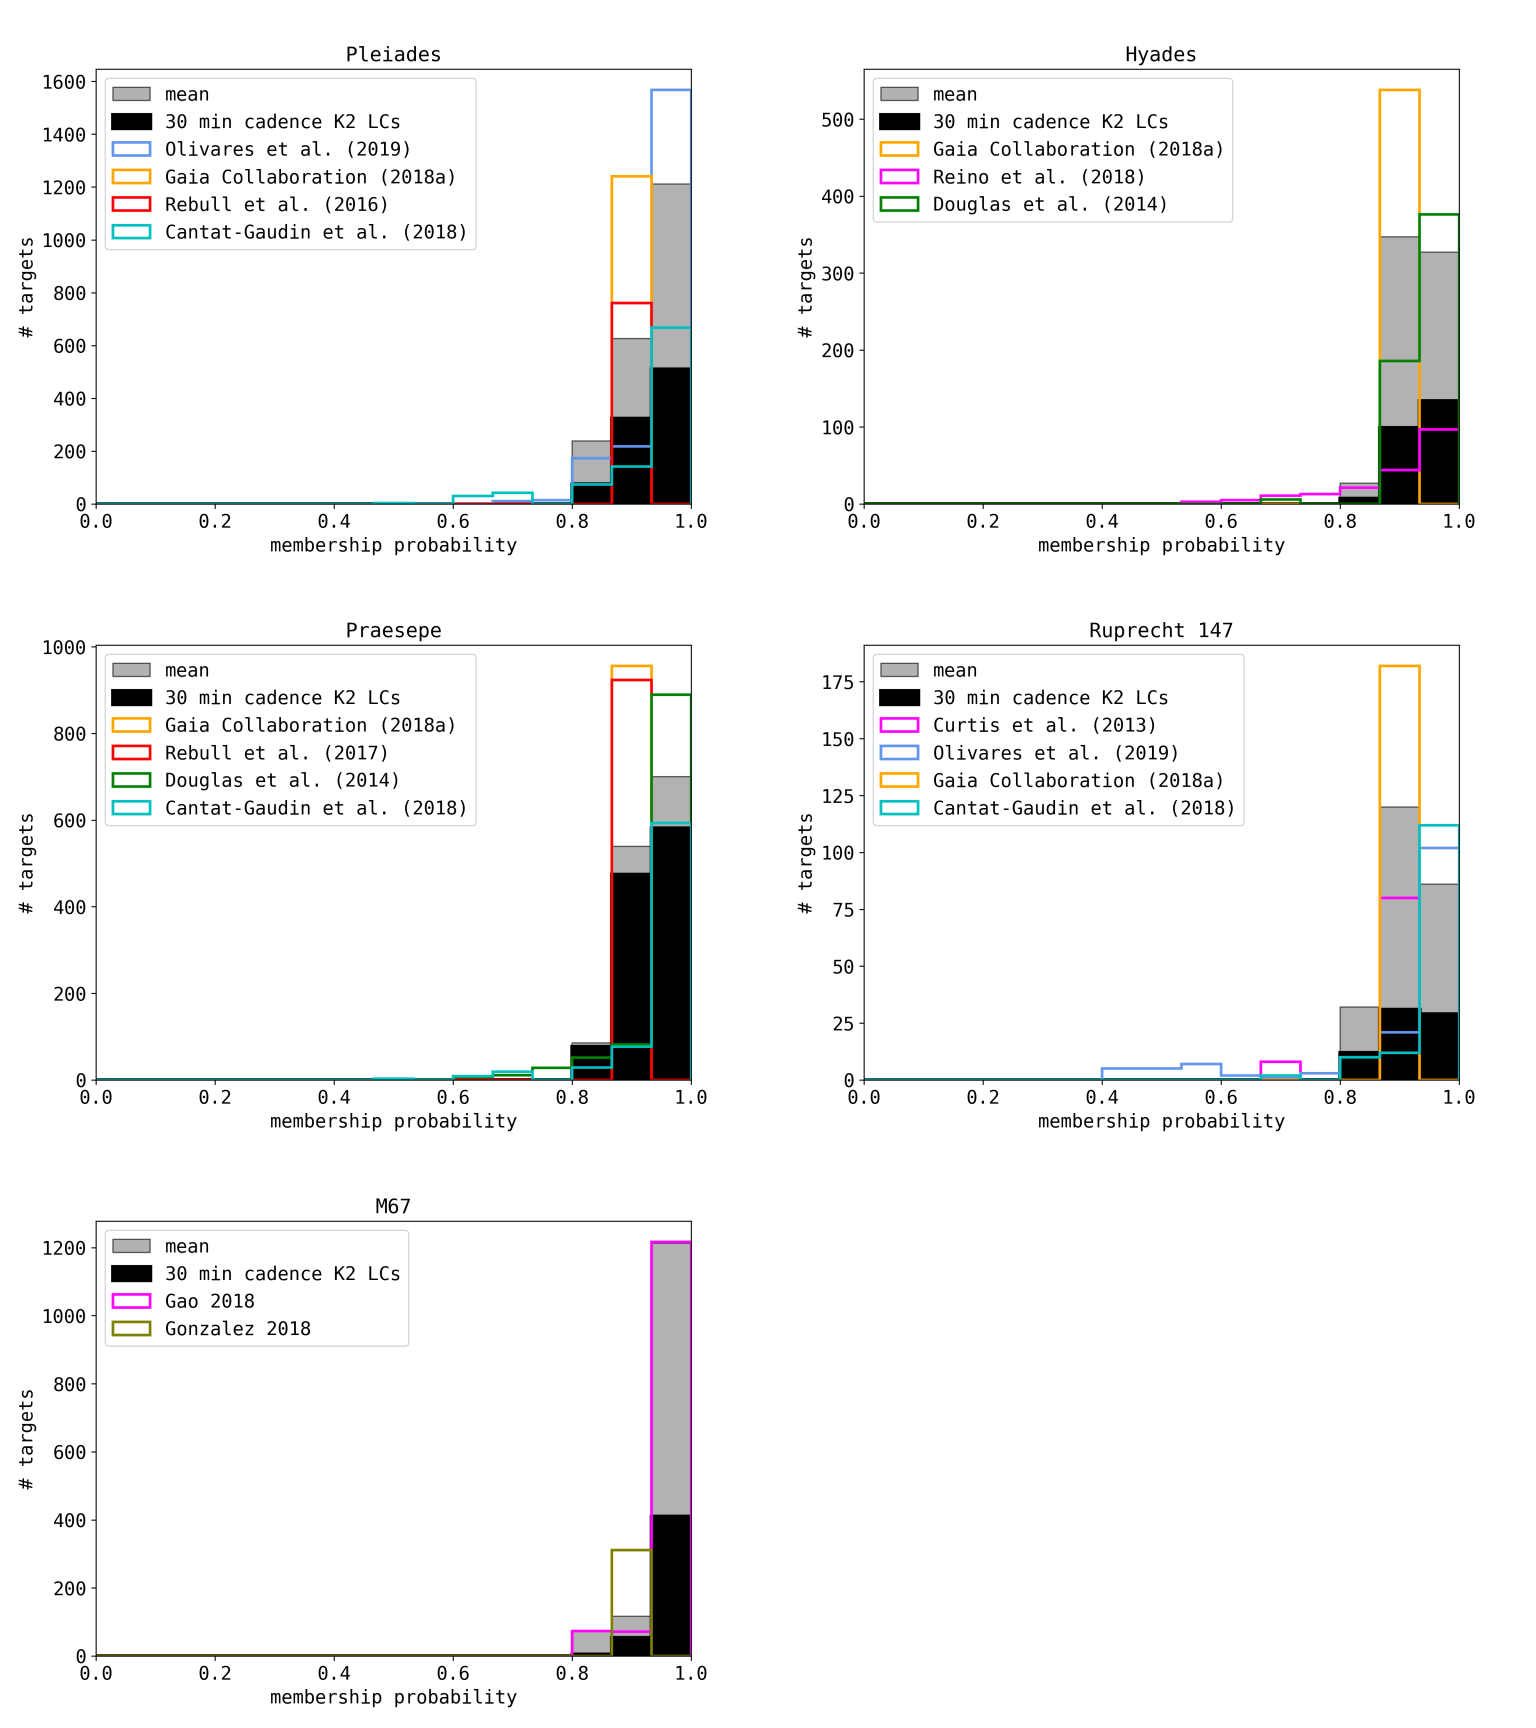
\includegraphics[width=\hsize]{pics/appendix/membership_histograms.png}
         \caption{Membership histograms.}
          \label{figure_app_memberships}
         % X panel: Power law exponent $\alpha_\mathrm{MK}$, fitting procedure follows Bauke (2007).
   \end{figure*}

%--------------------------------------------------------------------


\section{Cluster parameters}
\label{appendix0}

\begin{table*}
\caption{Non-exhaustive literature overview over OC parameters.}
\label{tab:app:oc_parameters}
\centering
\begin{tabular}{lllll}
\hline\hline
     cluster &                                source & distance [pc] &                            age [Myr] &                       [Fe/H] \\
\hline
% \textbf{M35}& \textbf{adopted in this work:}        &     861       & $ 147.5     \pm _{ 13.5}^{13.5   }$  & $-0.21         \pm 0.10  $   \\
% M35         &Bossini et al. (2019) \tablefootmark{a}&               & $ 402.7           \pm _{ 0.9}^{1.9}$ &                              \\
% M35         &             Cantat-Gaudin et al.(2018)&     861       &                                      &                              \\
% M35         &             Netopil et al. (2016)     &               &                                      &               -0.21          \\
% M35         &             Scholz et al. (2015)      &     830       &                           151        &                              \\
% M35         &             Geller et al. (2010)      &               &                           133        &                              \\
% M35         &             Meibom et al. (2009)      &               &  $ 147.5     \pm _{ 13.5}^{13.5   }$ &                              \\
% M35         &             Bragaglia and Tosi (2006) &     912       &                                      &                              \\
% M35         &  Steinhauser and Deliyannis (2004)    &               &                                      &  $-0.143        \pm 0.014 $ \\
% M35         &             Barrado (2001)            &               &                           180        &                              \\
% M35         &             Barrado et al. (2001)     &               &                                      &  $-0.21         \pm 0.10  $ \\
% M35         &             Sung and Bessel (1999)    &     832       &                                      &                              \\\hline
\textbf{Pleiades} & \textbf{adopted in this work:}   &     135.6     &  $ 135       \pm _{ 25}^{25       }$ & $ -0.037        \pm 0.026 $  \\
	    &\citet{bossini2019} \tablefootmark{a}  && $86.5 \pm _{ 2.4}^{6       }$        &                              \\
 	    &           \citet{cantat_gaudin_2018} &     135.6     &                                      &                              \\
 	    &             \citet{gossage2018}     &               &  $ 135       \pm _{ 25}^{25       }$ &                              \\
	    &            \citet{yen2018}            &     126.3     &  $ 141.3     \pm _{ 100}^{170     }$ &                              \\
 	    &            \citet{chelli2016}   &     139       &                                      &                              \\
 	    &  \citet{netopil_metallicities_2016}   &               &                                      &               -0.01          \\
	    &             \citet{dahm_reexamining_2015}              &               &  $ 112       \pm _{ 5}^{5         }$ &                              \\
 	    &            \citet{scholz2015}     &     130       &                           120        &                              \\
	    &        \citet{conrad2014}    &               &                                      &  $ -0.037        \pm 0.026 $ \\
	    &             \citet{melis2014}      &     136       &                                      &                              \\
			  &   \citet{bell_pre-main-sequence_2012}   &     135       &                           125        &                              \\\hline
\textbf{Hyades} & \textbf{adopted in this work:\tablefootmark{c}}     &               &  $ 690       \pm _{ 100}^{160     }$ &  $0.13  \pm 0.02$            \\	       	&             \citet{gaia_dr2_2018_hrd} &               &  $ 690       \pm _{ 100}^{160     }$ &                              \\
       &             \citet{gossage2018}     &               &                           680        &                              \\
       &             \citet{liu2016}        &               &                                      &  $               \pm 0.02  $ \\
       &             \citet{netopil_metallicities_2016}    &               &                                      &               0.13           \\
       &             \citet{taylor2005}  &               &                                      &  $ 0.103         \pm 0.008 $ \\
 %Hyades      &             Cummings et al. (2005)    &               &                                      &  $ 0.146         \pm 0.004 $ \\
       &            \citet{salaris_age_2004}    &               &  $650$                               &  $ 0.15$                      \\
       &             \citet{perryman1998}    &               &  $ 625       \pm _{ 50}^{50       }$ &                              \\\hline
 %Hyades      &             Martin et al. (1998)      &               &  $ 650       \pm _{ 70}^{70       }$ &                               
\textbf{Praesepe} & \textbf{adopted in this work:}   &     185.5     &  $ 750\pm _{7}^{ 3 }$                &              0.16            \\
     &               \citet{bossini2019}     &               &                 $ 750\pm _{7}^{ 3 }$ &                              \\
     &            \citet{cantat_gaudin_2018} &     185.5     &                                      &                              \\
     &               \citet{gossage2018}     &               &                           590        &                              \\
     &             \citet{yen2018}           &     183       &  $ 794       \pm _{ 269}^{253     }$ &                              \\
     &\citet{netopil_metallicities_2016}     &               &                                      &               0.16           \\
     &             \citet{scholz2015}    &     187       &                           832        &                              \\
     &             \citet{boesgaard2013}   &               &                                      &               0.12           \\
     &             \citet{boudreault_astrometric_2012}  &     160       &                           630        &                              \\
     &            \citet{salaris_age_2004}     &     175       &                           650        &                              \\\hline
\textbf{Ruprecht 147} & \textbf{adopted in this work:}    &     305       & $ 2650      \pm _{ 380}^{380     }$  & $ 0.08          \pm 0.07  $  \\
     &             \citet{bragaglia2018}   &               &                                      &  $ 0.08          \pm 0.07  $ \\
      &           \citet{cantat_gaudin_2018} &     305       &                                      &                              \\
      &             \citet{gaia_dr2_2018_hrd} &     309       &  $ 1995      \pm _{ 257}^{404     }$ &                              \\
     &             \citet{torres2018}     &     283       &  $ 2650      \pm _{ 380}^{380     }$ &                              \\
    &             \citet{curtis2016}\tablefootmark{b} &               &                                      &  $ 0.10          \pm 0.02  $ \\
     &           \citet{scholz2015}    &     270     &                           1953       &                              \\
     &             \citet{curtis2013}    &     300       &  $ 3125      \pm _{ 125}^{125     }$ &  $ 0.07          \pm 0.03  $ 
\\\hline  
\textbf{M67} & \textbf{adopted in this work:}        &     908       & $3639  \pm _{ 17}^{17      }$        & $ -0.102         \pm .081  $ \\
          &             \citet{bossini2019}       &               &   $3639  \pm _{ 17}^{17      }$      &                              \\
          & \citet{netopil_metallicities_2016}    &               &                                      &               0.03           \\
          &             \citet{scholz2015}    &               &  $ 3428      \pm _{ 72}^{147      }$ &                              \\
          &           \citet{conrad2014}     &               &                                      &  $ -0.102         \pm .081  $ \\
          &           \citet{dias_fitting_2012}      &     908       &                           4300       &                              \\
          &             \citet{onehag2011}    &     880       &                           4200       &               0.02           \\
          & \citet{salaris_age_2004}           &                   & $ 4300      \pm _{500}^{500}$    &       $0.02\pm 0.06$               \\\hline
\end{tabular}


\tablefoot{
\tablefoottext{a}{Bossini et al. (2019) noted some caveats for their determination of ages of young clusters, for which they used Gaia DR2 photometry for isochrone fitting.}
\tablefoottext{b}{Curtis (2016) reanalysed HIRES spectra using an improved spectroscopic method as compared to Curtis et al. (2013).
\tablefoottext{c}{We did not adopt a mean value for the Hyades distance because the cluster members are on average closer than 50 pc.}}
}
\end{table*}

%The identical ages for Paresepe in Yen+ and Kharchenko+ are coincidental


\section{Broadband photometry: quality cuts and conversions}
\label{appendix_photometry}
We required \texttt{flux}/\texttt{flux\_error}$\geq 10$ for Gaia G, BP, and RP bands. We require that the 2MASS measurements for J, H, and K to be "A". "A" means that measurements had $S/N>10$ and $\sigma<0.11$. For PanSTARRS photometry, we required that the \texttt{QF\_OBJ\_GOOD} quality filter flag was set. %We required flags 8 or 16 or 32 in the \texttt{gFlags}~(and respective flags for r,i,z, and y) from \texttt{ObjectFilterFlags} to be set for each band. 8 indicates that observation were made on a photometric night. 16 and 32 verify that PS1 photometry was obtained.
\\
SDSS and PS1 \textit{ugrizy} bands are similar but not identical, but can be converted using Table 2 in~\citet{finkbeiner_ps1tosdss_2016}.
\section{Pixel saturation}
Resolve different levels of pixel saturation (>1, >10) and how they contribute to the deviations from the single power law at the highest energies.
\section{Solar system objects}
Solar system objects (SSOs) produce brightness excursions in K2 light curves that can closely resemble flare signatures. Often, they can be distinguished by their symmetric rise and decay shape as contrasted with the typical fast-rise gradual decay flare shape~\citep{davenport_kepler_2014}.
M. H. Christiansen and colleagues developed a routine called \texttt{SkyBoT} that matches positions and times to passages of SSOs listed in YYY. RA, declination, start, stop, and mid epochs of flares in BKJD are the input parameters. We excluded all flare candidates that occurred within X minutes of a SSO passage at the star's position. This procedure removed ZZ\% of all flare candidates. In the case of high energy flares, we confirmed the passage by manually inspecting the pixel file with the \texttt{lightkurve} \texttt{interact} function for TargetPixelFiles.
\section{Universality of power law exponent $\alpha$}
We compiled a exhaustive (?) table of previous work where power laws were fitted to FFDs using different methods. Table \ref{app_powerlaw_literature} lists the overview. While particular studies consistently find values above or below $\alpha\approx2$, the comparison of different studies points towards unresolved systematic errors in all these studies. \begin{table*}
\caption{Literature overview over power law fitting approaches to FFDs.}
\label{app_powerlaw_literature}
\centering

\begin{tabular}{lL{6cm}L{4cm}l}
%ONLY COPY BELOW THIS LINE
\toprule
                      Who &                                                                                  method &                                                          data &      $\alpha-1$ \\
\midrule
  Hawley et al. (2014)    &    LSq with Poisson uncertainty, increase the low energy limit until the fit is robust  &                                                               &     .95 (binned), 1.01 (cumulative)      \\
  Davenport (2016)        &            weighted LSq, asymmetric Poisson confidence intervals following Gehrels1986  &                                                               &                 \\
  Gizis  (2017)           &    de-biased MLE (Arnold2015), weight each point with sqrt(N) in each bin (Clauset+2009 &                                                              22 flares on one M7 UCD &   .6-1. (31-33 erg)              \\
  Paudel et al. (2018)    &                               ML from a paper in 2010, used emcee (Foreman-Mackey2013)  &                                                               &                 \\
  Lacy (1976)             &                                                                  graphical, linear LSq  &                                        386 flares on UV Cetis &         .43-1.  \\
  Güdel et al.(2003)      &      -                                                                                   &                                                               &                 \\
  Davenport et al. (2012) &              Fit $\log_{10} Y = \alpha + (\beta \log_{10} X)(10 -\gamma /(X+\delta) )$  &  $\sim$50,000 M dwarfs from SDSS and 1321 M dwarfs from 2MASS &          .9-2.1 \\
  Lurie et al. (2015)     &   Bayesian Markov chain Monte Carlo based algorithm (Kelly 2007) for linear regression  &                                                2 dMe5 dwarfs  &        .92-1.03 \\
  Audard et al. (2000)    &                                                      Crawford+1970 MLE (Jauncey-style)  &                    EUVE 12 F-M type stars, 10-20 flares each  &        .46-1.61 \\
  Shakhovskaia (1989)     &                      linear representation, power laws from Gershberg/Shakhovskaya1983  &                                     30-40 dK0-dM8, 200 flares &          .4-1.4 \\
  Yang et al. (2017)      &                                                                            binned FFDs  &                 103187 flares on 540 M-type dwarfs in Kepler  &   1.07 +/- 0.35 \\
  Howard et al. (2018)    & fit a cumulative power law, MCMC for uncertainties &575 flares on 284 stars & 0.84-1.34\\
  Hilton et al. (2011) &&&.63-.83\\ 
\bottomrule
\end{tabular}

\end{table*}

\section{Expanding the likelihood}
The rate $\lambda_2$ of flares with energies larger than $S_2$ is given in \citet{wheatland_flaresbayes_2004} as
\begin{equation}
\label{eqn4}
    \lambda_2 = \lambda_1 \cdot \left(\dfrac{S_1}{S_2}\right)^{\alpha-1}.
\end{equation}
$S_1$ denotes the energy above which all flares are detected. $\lambda_1$ is the corresponding rate. $\alpha$ remains the power law exponent of the flare frequency distribution.
\\
We are also given the posterior distribution for the rate $\lambda_2$ of flares above $S_2$ in Eq. (20) in \citet{wheatland_flaresbayes_2004}:
\begin{eqnarray}
\label{eqn20}
P_2(\lambda_2) &=& \displaystyle \int_{1}^{\infty} \mathrm{d}\alpha \int_{0}^{\infty} \mathrm{d}\lambda_1 \delta\left(\lambda_2 - \lambda_1 \cdot \left( \dfrac{S_1}{S_2} \right)^{\alpha-1}\right)\nonumber \\
&&\cdot P_1(\lambda_1) \cdot P_{\alpha}(\alpha)
\end{eqnarray}
As we have additional information in the form of uncertainties in our data $S=\{S_i,\lambda_i,\sigma_{S,i}\}$, we can expand Eq. \ref{eqn20} with this knowledge. Assuming that the observed flare energies $S_i$ with cumulative rates $\lambda_i$ are distributed around the real flare energies $S_{0,i}$ with Gaussian uncertainties $\sigma_{S,i}$, we can define:
\begin{eqnarray}
    \label{pSi}
    p(S_i | \lambda_1, \alpha, \sigma_{S,i})
    &=& \dfrac{1}{2\pi \sqrt{\sigma_{S,i}}} \mathrm{e}^{-\dfrac{\left(S_i - S_{0,i}\right)^2}{2\sigma_{S,i}^2}}\nonumber\\
    &=& \dfrac{1}{2\pi \sqrt{\sigma_{S,i}}} \mathrm{e}^{-\dfrac{\left(S_i - S_1\left(\dfrac{\lambda_i}{\lambda_1}\right)^{-1/(\alpha-1)}\right)^2}{2\sigma_{S,i}^2}}
\end{eqnarray}
We assume in Eq. \ref{pSi} that uncertainties on $\lambda_1$ are negligible. Eq. \ref{eqn20} then reads:
\begin{eqnarray}
\label{eqn201}
P_2(\lambda_2) &=& \displaystyle \int_{1}^{\infty} \mathrm{d}\alpha \int_{0}^{\infty} \mathrm{d}\lambda_1 \delta\left(\lambda_2 - \lambda_1 \cdot \left( \dfrac{S_1}{S_2} \right)^{\alpha-1}\right)\nonumber \\
&&\cdot P_1(\lambda_1) \cdot P_{\alpha}(\alpha) \cdot P_S(S| \lambda_1, \alpha, \sigma_S)
\end{eqnarray}
with
\begin{equation}
    P_S(S | \lambda_1, \alpha, \sigma_S) = C\displaystyle \prod_{i=1}^M p(S_i | \lambda_1, \alpha, \sigma_{S,i}).
\end{equation}
$C$ absorbs the normalization, or evidence term.
\\
Following \citet{wheatland_flaresbayes_2004}, we marginalize over $\lambda_1$ using the $\delta$ function in \ref{eqn201} to obtain
\begin{eqnarray}
\label{eqn21}
P_2(\lambda_2) &=& \displaystyle \int_{1}^{\infty} \mathrm{d}\alpha \cdot P_1\left(\lambda_2 \cdot\left(\dfrac{S_2}{S_1}\right)^{\alpha-1}\right) \cdot P_{\alpha}(\alpha)\nonumber\\
&&\cdot P_S\left(S| \lambda_2 \cdot\left(\dfrac{S_2}{S_1}\right)^{\alpha-1}, \alpha, \sigma_S\right)
\end{eqnarray}
Transforming $P_S$ into a function of $\epsilon$ with $\lambda_1=-\ln(1-\epsilon)/\Delta T$ yields:
\begin{eqnarray}
    P_S(S | \epsilon, \alpha, \sigma_S) &=& C \displaystyle \prod_{i=1}^M p(S_i | \epsilon, \alpha, \sigma_{S,i})\nonumber\\
    &=& \dfrac{C}{\Delta T(1-\epsilon)}\nonumber\\
    &&\cdot \displaystyle \prod_{i=1}^M \left[\dfrac{1}{2\pi \sqrt{\sigma_{S,i}}}\mathrm{e}^{-\dfrac{\left(S_i - S_2\left(\dfrac{-\ln(1-\epsilon)}{\Delta T\lambda_i}\right)^{1/(\alpha-1)}\right)^2}{2\sigma_{S,i}^2}}\right]
\end{eqnarray}
Finally, $P_S$ enters the joint posterior distribution from Eq. \ref{joint_posterior}, that becomes
\begin{eqnarray}
\label{joint_posterior2}
p(\epsilon, \alpha) &=& C \cdot\, (-\ln(1 - \epsilon)^{M})\nonumber\\
                    && \cdot\, (\alpha-1)^M \cdot\, \Gamma(\alpha) \left[\dfrac{(S_2 / S_1)^{M+1}}{\pi} \right]^{\alpha}\nonumber\\
                    && \cdot\, (1-\epsilon)^{(T / \Delta T) \,\cdot\, (S_2 /S_1)^{\alpha-1} -1 }\nonumber\\
                    &&\cdot P_S(S | \epsilon, \alpha, \sigma_S).
\end{eqnarray}
\end{appendix}
\end{document}


%%%%%%%%%%%%%%%%%%%%%%%%%%%%%%%%%%%%%%%%%%%%%%%%%%%%%%%%%%%%%%
Examples for figures using graphicx
A guide "Using Imported Graphics in LaTeX2e"  (Keith Reckdahl)
is available on a lot of LaTeX public servers or ctan mirrors.
The file is : epslatex.pdf
%%%%%%%%%%%%%%%%%%%%%%%%%%%%%%%%%%%%%%%%%%%%%%%%%%%%%%%%%%%%%%

%_____________________________________________________________
%                 A figure as large as the width of the column
%-------------------------------------------------------------
   \begin{figure}
   \centering
   \includegraphics[width=\hsize]{empty.eps}
      \caption{Vibrational stability equation of state
               $S_{\mathrm{vib}}(\lg e, \lg \rho)$.
               $>0$ means vibrational stability.
              }
         \label{FigVibStab}
   \end{figure}
%
%_____________________________________________________________
%                                    One column rotated figure
%-------------------------------------------------------------
   \begin{figure}
   \centering
   \includegraphics[angle=-90,width=3cm]{empty.eps}
      \caption{Vibrational stability equation of state
               $S_{\mathrm{vib}}(\lg e, \lg \rho)$.
               $>0$ means vibrational stability.
              }
         \label{FigVibStab}
   \end{figure}
%
%_____________________________________________________________
%                        Figure with caption on the right side
%-------------------------------------------------------------
   \begin{figure}
   \sidecaption
   \includegraphics[width=3cm]{empty.eps}
      \caption{Vibrational stability equation of state
               $S_{\mathrm{vib}}(\lg e, \lg \rho)$.
               $>0$ means vibrational stability.
              }
         \label{FigVibStab}
   \end{figure}
%
%_____________________________________________________________
%
%_____________________________________________________________
%                                Figure with a new BoundingBox
%-------------------------------------------------------------
   \begin{figure}
   \centering
   \includegraphics[bb=10 20 100 300,width=3cm,clip]{empty.eps}
      \caption{Vibrational stability equation of state
               $S_{\mathrm{vib}}(\lg e, \lg \rho)$.
               $>0$ means vibrational stability.
              }
         \label{FigVibStab}
   \end{figure}
%
%_____________________________________________________________
%
%_____________________________________________________________
%                                      The "resizebox" command
%-------------------------------------------------------------
   \begin{figure}
   \resizebox{\hsize}{!}
            {\includegraphics[bb=10 20 100 300,clip]{empty.eps}
      \caption{Vibrational stability equation of state
               $S_{\mathrm{vib}}(\lg e, \lg \rho)$.
               $>0$ means vibrational stability.
              }}
         \label{FigVibStab}
   \end{figure}
%
%______________________________________________________________
%
%_____________________________________________________________
%                                             Two column Figure
%-------------------------------------------------------------
   \begin{figure*}
   \resizebox{\hsize}{!}
            {\includegraphics[bb=10 20 100 300,clip]{empty.eps}
      \caption{Vibrational stability equation of state
               $S_{\mathrm{vib}}(\lg e, \lg \rho)$.
               $>0$ means vibrational stability.
              }}
         \label{FigVibStab}
   \end{figure*}
%
%______________________________________________________________
%
%_____________________________________________________________
%                                             Simple A&A Table
%_____________________________________________________________
%
\begin{table}
\caption{Nonlinear Model Results}             % title of Table
\label{table:1}      % is used to refer this table in the text
\centering                          % used for centering table
\begin{tabular}{c c c c}        % centered columns (4 columns)
\hline\hline                 % inserts double horizontal lines
HJD & $E$ & Method\#2 & Method\#3 \\    % table heading
\hline                        % inserts single horizontal line
   1 & 50 & $-837$ & 970 \\      % inserting body of the table
   2 & 47 & 877    & 230 \\
   3 & 31 & 25     & 415 \\
   4 & 35 & 144    & 2356 \\
   5 & 45 & 300    & 556 \\
\hline                                   %inserts single line
\end{tabular}
\end{table}
%
%_____________________________________________________________
%                                             Two column Table
%_____________________________________________________________
%
\begin{table*}
\caption{Nonlinear Model Results}
\label{table:1}
\centering
\begin{tabular}{c c c c l l l }     % 7 columns
\hline\hline
                      % To combine 4 columns into a single one
HJD & $E$ & Method\#2 & \multicolumn{4}{c}{Method\#3}\\
\hline
   1 & 50 & $-837$ & 970 & 65 & 67 & 78\\
   2 & 47 & 877    & 230 & 567& 55 & 78\\
   3 & 31 & 25     & 415 & 567& 55 & 78\\
   4 & 35 & 144    & 2356& 567& 55 & 78 \\
   5 & 45 & 300    & 556 & 567& 55 & 78\\
\hline
\end{tabular}
\end{table*}
%
%-------------------------------------------------------------
%                                          Table with notes
%-------------------------------------------------------------
%
% A single note
\begin{table}
\caption{\label{t7}Spectral types and photometry for stars in the
  region.}
\centering
\begin{tabular}{lccc}
\hline\hline
Star&Spectral type&RA(J2000)&Dec(J2000)\\
\hline
69           &B1\,V     &09 15 54.046 & $-$50 00 26.67\\
49           &B0.7\,V   &*09 15 54.570& $-$50 00 03.90\\
LS~1267~(86) &O8\,V     &09 15 52.787&11.07\\
24.6         &7.58      &1.37 &0.20\\
\hline
LS~1262      &B0\,V     &09 15 05.17&11.17\\
MO 2-119     &B0.5\,V   &09 15 33.7 &11.74\\
LS~1269      &O8.5\,V   &09 15 56.60&10.85\\
\hline
\end{tabular}
\tablefoot{The top panel shows likely members of Pismis~11. The second
panel contains likely members of Alicante~5. The bottom panel
displays stars outside the clusters.}
\end{table}
%
% More notes
%
\begin{table}
\caption{\label{t7}Spectral types and photometry for stars in the
  region.}
\centering
\begin{tabular}{lccc}
\hline\hline
Star&Spectral type&RA(J2000)&Dec(J2000)\\
\hline
69           &B1\,V     &09 15 54.046 & $-$50 00 26.67\\
49           &B0.7\,V   &*09 15 54.570& $-$50 00 03.90\\
LS~1267~(86) &O8\,V     &09 15 52.787&11.07\tablefootmark{a}\\
24.6         &7.58\tablefootmark{1}&1.37\tablefootmark{a}   &0.20\tablefootmark{a}\\
\hline
LS~1262      &B0\,V     &09 15 05.17&11.17\tablefootmark{b}\\
MO 2-119     &B0.5\,V   &09 15 33.7 &11.74\tablefootmark{c}\\
LS~1269      &O8.5\,V   &09 15 56.60&10.85\tablefootmark{d}\\
\hline
\end{tabular}
\tablefoot{The top panel shows likely members of Pismis~11. The second
panel contains likely members of Alicante~5. The bottom panel
displays stars outside the clusters.\\
\tablefoottext{a}{Photometry for MF13, LS~1267 and HD~80077 from
Dupont et al.}
\tablefoottext{b}{Photometry for LS~1262, LS~1269 from
Durand et al.}
\tablefoottext{c}{Photometry for MO2-119 from
Mathieu et al.}
}
\end{table}
%
%-------------------------------------------------------------
%                                       Table with references
%-------------------------------------------------------------
%
\begin{table*}[h]
 \caption[]{\label{nearbylistaa2}List of nearby SNe used in this work.}
\begin{tabular}{lccc}
 \hline \hline
  SN name &
  Epoch &
 Bands &
  References \\
 &
  (with respect to $B$ maximum) &
 &
 \\ \hline
1981B   & 0 & {\it UBV} & 1\\
1986G   &  $-$3, $-$1, 0, 1, 2 & {\it BV}  & 2\\
1989B   & $-$5, $-$1, 0, 3, 5 & {\it UBVRI}  & 3, 4\\
1990N   & 2, 7 & {\it UBVRI}  & 5\\
1991M   & 3 & {\it VRI}  & 6\\
\hline
\noalign{\smallskip}
\multicolumn{4}{c}{ SNe 91bg-like} \\
\noalign{\smallskip}
\hline
1991bg   & 1, 2 & {\it BVRI}  & 7\\
1999by   & $-$5, $-$4, $-$3, 3, 4, 5 & {\it UBVRI}  & 8\\
\hline
\noalign{\smallskip}
\multicolumn{4}{c}{ SNe 91T-like} \\
\noalign{\smallskip}
\hline
1991T   & $-$3, 0 & {\it UBVRI}  &  9, 10\\
2000cx  & $-$3, $-$2, 0, 1, 5 & {\it UBVRI}  & 11\\ %
\hline
\end{tabular}
\tablebib{(1)~\citept{branch83};
(2) \citept{phillips87}; (3) \citept{barbon90}; (4) \citept{wells94};
(5) \citept{mazzali93}; (6) \citept{gomez98}; (7) \citept{kirshner93};
(8) \citept{patat96}; (9) \citept{salvo01}; (10) \citept{branch03};
(11) \citept{jha99}.
}
\end{table*}
%_____________________________________________________________
%                      A rotated Two column Table in landscape
%-------------------------------------------------------------
\begin{sidewaystable*}
\caption{Summary for ISOCAM sources with mid-IR excess
(YSO candidates).}\label{YSOtable}
\centering
\begin{tabular}{crrlcl}
\hline\hline
ISO-L1551 & $F_{6.7}$~[mJy] & $\alpha_{6.7-14.3}$
& YSO type$^{d}$ & Status & Comments\\
\hline
  \multicolumn{6}{c}{\it New YSO candidates}\\ % To combine 6 columns into a single one
\hline
  1 & 1.56 $\pm$ 0.47 & --    & Class II$^{c}$ & New & Mid\\
  2 & 0.79:           & 0.97: & Class II ?     & New & \\
  3 & 4.95 $\pm$ 0.68 & 3.18  & Class II / III & New & \\
  5 & 1.44 $\pm$ 0.33 & 1.88  & Class II       & New & \\
\hline
  \multicolumn{6}{c}{\it Previously known YSOs} \\
\hline
  61 & 0.89 $\pm$ 0.58 & 1.77 & Class I & \object{HH 30} & Circumstellar disk\\
  96 & 38.34 $\pm$ 0.71 & 37.5& Class II& MHO 5          & Spectral type\\
\hline
\end{tabular}
\end{sidewaystable*}
%_____________________________________________________________
%                      A rotated One column Table in landscape
%-------------------------------------------------------------
\begin{sidewaystable}
\caption{Summary for ISOCAM sources with mid-IR excess
(YSO candidates).}\label{YSOtable}
\centering
\begin{tabular}{crrlcl}
\hline\hline
ISO-L1551 & $F_{6.7}$~[mJy] & $\alpha_{6.7-14.3}$
& YSO type$^{d}$ & Status & Comments\\
\hline
  \multicolumn{6}{c}{\it New YSO candidates}\\ % To combine 6 columns into a single one
\hline
  1 & 1.56 $\pm$ 0.47 & --    & Class II$^{c}$ & New & Mid\\
  2 & 0.79:           & 0.97: & Class II ?     & New & \\
  3 & 4.95 $\pm$ 0.68 & 3.18  & Class II / III & New & \\
  5 & 1.44 $\pm$ 0.33 & 1.88  & Class II       & New & \\
\hline
  \multicolumn{6}{c}{\it Previously known YSOs} \\
\hline
  61 & 0.89 $\pm$ 0.58 & 1.77 & Class I & \object{HH 30} & Circumstellar disk\\
  96 & 38.34 $\pm$ 0.71 & 37.5& Class II& MHO 5          & Spectral type\\
\hline
\end{tabular}
\end{sidewaystable}
%
%_____________________________________________________________
%                              Table longer than a single page
%-------------------------------------------------------------
% All long tables will be placed automatically at the end, after
%                                        \end{thebibliography}
%
\begin{longtab}
\begin{longtable}{lllrrr}
\caption{\label{kstars} Sample stars with absolute magnitude}\\
\hline\hline
Catalogue& $M_{V}$ & Spectral & Distance & Mode & Count Rate \\
\hline
\endfirsthead
\caption{continued.}\\
\hline\hline
Catalogue& $M_{V}$ & Spectral & Distance & Mode & Count Rate \\
\hline
\endhead
\hline
\endfoot
%%
Gl 33    & 6.37 & K2 V & 7.46 & S & 0.043170\\
Gl 66AB  & 6.26 & K2 V & 8.15 & S & 0.260478\\
Gl 68    & 5.87 & K1 V & 7.47 & P & 0.026610\\
         &      &      &      & H & 0.008686\\
Gl 86
\footnote{Source not included in the HRI catalog. See Sect.~5.4.2 for details.}
         & 5.92 & K0 V & 10.91& S & 0.058230\\
\end{longtable}
\end{longtab}
%
%_____________________________________________________________
%                              Table longer than a single page
%                                             and in landscape
%  In the preamble, use:       \usepackage{lscape}
%-------------------------------------------------------------
% All long tables will be placed automatically at the end, after
%                                        \end{thebibliography}
%
\begin{longtab}
\begin{landscape}
\begin{longtable}{lllrrr}
\caption{\label{kstars} Sample stars with absolute magnitude}\\
\hline\hline
Catalogue& $M_{V}$ & Spectral & Distance & Mode & Count Rate \\
\hline
\endfirsthead
\caption{continued.}\\
\hline\hline
Catalogue& $M_{V}$ & Spectral & Distance & Mode & Count Rate \\
\hline
\endhead
\hline
\endfoot
%%
Gl 33    & 6.37 & K2 V & 7.46 & S & 0.043170\\
Gl 66AB  & 6.26 & K2 V & 8.15 & S & 0.260478\\
Gl 68    & 5.87 & K1 V & 7.47 & P & 0.026610\\
         &      &      &      & H & 0.008686\\
Gl 86
\footnote{Source not included in the HRI catalog. See Sect.~5.4.2 for details.}
         & 5.92 & K0 V & 10.91& S & 0.058230\\
\end{longtable}
\end{landscape}
\end{longtab}
%
% Online Material
%_____________________________________________________________
%        Online appendices have to be placed at the end, after
%                                        \end{thebibliography}
%-------------------------------------------------------------
%\end{thebibliography}

\Online

\begin{appendix} %First online appendix
\section{Background galaxy number counts and shear noise-levels}
Because the optical images used in this analysis...

\begin{figure*}
\centering
\includegraphics[width=16.4cm,clip]{1787f24.ps}
\caption{Plotted above...}
\label{appfig}
\end{figure*}

Because the optical images...
\end{appendix}

\begin{appendix} %Second online appendix
These studies, however, have faced...
\end{appendix}

%\end{document}
%
%_____________________________________________________________
%        Some tables or figures are in the printed version and
%                      some are only in the electronic version
%-------------------------------------------------------------
%
% Leave all the tables or figures in the text, at their right place
% and use the commands \onlfig{} and \onltab{}. These elements
% will be automatically placed at the end, in the section
% Online material.

\documentclass{aa}
...
\begin{document}
text of the paper...
\begin{figure*}%f1
\includegraphics[width=10.9cm]{1787f01.eps}
\caption{Shown in greyscale is a...}
\label{cl12301}
\end{figure*}
...
from the intrinsic ellipticity distribution.
% Figure 2 available electronically only
\onlfig{
\begin{figure*}%f2
\includegraphics[width=11.6cm]{1787f02.eps}
\caption {Shown in greyscale...}
\label{cl1018}
\end{figure*}
}

% Figure 3 available electronically only
\onlfig{
\begin{figure*}%f3
\includegraphics[width=11.2cm]{1787f03.eps}
\caption{Shown in panels...}
\label{cl1059}
\end{figure*}
}

\begin{figure*}%f4
\includegraphics[width=10.9cm]{1787f04.eps}
\caption{Shown in greyscale is...}
\label{cl1232}
\end{figure*}

\begin{table}%t1
\caption{Complexes characterisation.}\label{starbursts}
\centering
\begin{tabular}{lccc}
\hline \hline
Complex & $F_{60}$ & 8.6 &  No. of  \\
...
\hline
\end{tabular}
\end{table}
The second method produces...

% Figure 5 available electronically only
\onlfig{
\begin{figure*}%f5
\includegraphics[width=11.2cm]{1787f05.eps}
\caption{Shown in panels...}
\label{cl1238}
\end{figure*}
}

As can be seen, in general the deeper...
% Table 2 available electronically only
\onltab{
\begin{table*}%t2
\caption{List of the LMC stellar complexes...}\label{Properties}
\centering
\begin{tabular}{lccccccccc}
\hline  \hline
Stellar & RA & Dec & ...
...
\hline
\end{tabular}
\end{table*}
}

% Table 3 available electronically only
\onltab{
\begin{table*}%t3
\caption{List of the derived...}\label{IrasFluxes}
\centering
\begin{tabular}{lcccccccccc}
\hline \hline
Stellar & $f12$ & $L12$ &...
...
\hline
\end{tabular}
\end{table*}
}
\end{document}
%
%-------------------------------------------------------------
%     For the online material, table longer than a single page
%                 In the preamble for landscape case, use :
%                                          \usepackage{lscape}
%-------------------------------------------------------------
\documentclass{aa}
\usepackage[varg]{txfonts}
\usepackage{graphicx}
\usepackage{lscape}

\begin{document}
text of the paper
% Table will be print automatically at the end, in the section Online material.
\onllongtab{
\begin{longtable}{lrcrrrrrrrrl}
\caption{Line data and abundances ...}\\
\hline
\hline
Def & mol & Ion & $\lambda$ & $\chi$ & $\log gf$ & N & e &  rad & $\delta$ & $\delta$
red & References \\
\hline
\endfirsthead
\caption{Continued.} \\
\hline
Def & mol & Ion & $\lambda$ & $\chi$ & $\log gf$ & B & C &  rad & $\delta$ & $\delta$
red & References \\
\hline
\endhead
\hline
\endfoot
\hline
\endlastfoot
A & CH & 1 &3638 & 0.002 & $-$2.551 &  &  &  & $-$150 & 150 &  Jorgensen et al. (1996) \\
\end{longtable}
}% End onllongtab

% Or for landscape, large table:

\onllongtab{
\begin{landscape}
\begin{longtable}{lrcrrrrrrrrl}
...
\end{longtable}
\end{landscape}
}% End onllongtab
\end{document}
